\documentclass[conference]{IEEEtran}
\IEEEoverridecommandlockouts
% The preceding line is only needed to identify funding in the first footnote. If that is unneeded, please comment it out.
%Template version as of 6/27/2024

\usepackage{cite}
\usepackage{amsmath,amssymb,amsfonts}
\usepackage{algorithmic}
\usepackage{graphicx}
\usepackage{textcomp}
\usepackage{xcolor}
\usepackage{multirow}
\usepackage{array}
\usepackage{url}
\usepackage{tikz}
\usetikzlibrary{positioning,arrows.meta,calc}
\usepackage{xr}
\externaldocument[M-]{paper}

\def\BibTeX{{\rm B\kern-.05em{\sc i\kern-.025em b}\kern-.08em
    T\kern-.1667em\lower.7ex\hbox{E}\kern-.125emX}}
\begin{document}

\title{Supplementary Material: Entropy-Gated Triplet Learning and a Patient-History Markov Prior for Long-Tailed Multi-Label Chest X-Ray Classification}

\author{
\IEEEauthorblockN{Dr. Christian Wagner}
\IEEEauthorblockA{\textit{Professor of Computer Science}\\
The University of Nottingham\\
Nottingham, United Kingdom\\
Christian.Wagner@nottingham.ac.uk}
\and
\IEEEauthorblockN{Dr. Shreyank Narayana Gowda}
\IEEEauthorblockA{\textit{Assistant Professor}\\
The University of Nottingham\\
Nottingham, United Kingdom\\
Shreyank.NarayanaGowda@nottingham.ac.uk}
\and
\IEEEauthorblockN{Dr. Nguyen Trung Ky}
\IEEEauthorblockA{\textit{Professor of Computer Science}\\
International University - VNU\\
Ho Chi Minh City, Viet Nam\\
ntky@hcmiu.edu.vn}
\and
\IEEEauthorblockN{Ned Pham}
\IEEEauthorblockA{\textit{Student}\\
The University of Nottingham\\
Nottingham, United Kingdom\\
thien.pham@nottingham.ac.uk}
\and
\IEEEauthorblockN{Huy Pham}
\IEEEauthorblockA{\textit{Student}\\
International University - VNU\\
Ho Chi Minh City, Viet Nam\\
ititiu20216@student.hcmiu.edu.vn}
}

\maketitle

\renewcommand{\thesection}{S\arabic{section}}
\renewcommand{\thetable}{S\arabic{table}}
\renewcommand{\thefigure}{S\arabic{figure}}
\renewcommand{\theequation}{S\arabic{equation}}
\section*{About this supplement}
This supplement accompanies the main paper. Section, equation, table and figure numbers without an ``S'' prefix refer to the main paper. Sections~\ref{s:corr}--\ref{s:mat} give the implementation corrections, the full progression of the corrected implementation (v3), and the Stage-1 maturity and triplet-utilization results. Sections~\ref{s:mkmethod}--\ref{s:disc} give the full method, setup and results of the Markov priors tested on top of the entropy-gated model, the PadChest metadata analysis, the validation-proxy audit, and reproducibility notes. All numbers are on the internal validation fold unless stated. Table~\ref{tab:names} maps the model names of the main paper to the names used below and to the code and jobs behind them.

\begin{table}[htbp]
\caption{Model names in the main paper, the names used in this supplement, and the code and Slurm jobs behind them.}
\begin{center}
\resizebox{\linewidth}{!}{%
\footnotesize
\begin{tabular}{|l|l|l|}
\hline
\textbf{Main paper} & \textbf{This supplement} & \textbf{Code / jobs} \\
\hline
EGT, initial implementation & original code / implementation & \path{train_2_v2.py} (Aug.~2026 version); 43047--43051 \\
EGT, corrected implementation & v3 (512~px seed sweep) & \path{train_2_v3.py}; seed sweep \\
EGT-768 & v3, 768~px, SWA & 49000 (seed 42), 48999 (seed 1024) \\
EGT-1024 & v3, 1024~px, SWA & 48997 \\
EGT ensemble & greedy three-model ensemble & \path{analysis/ens_select.py}; members 49000, 48997, 47094 \\
EGT-768 + Markov prior & in-network patient-history prior & \path{train_2_v5.py}; 49375, 49376 \\
post-prediction fusion & patient HMM, arms H0--H5 & \path{analysis/markov_hmm_check.py}; 49445 \\
\hline
\end{tabular}}
\label{tab:names}
\end{center}
\end{table}

\section{Implementation Corrections}
\label{s:corr}\label{sec:corrections}
Tables~\ref{M-m:tab-entropy} and~\ref{tab2} were produced by our original Stage-2 code (Slurm jobs 43047--43051 for Table~\ref{M-m:tab-entropy}, 2026-08-27). An audit of that code against this paper found five differences, which we list rather than re-describe the method around them:
\begin{enumerate}
\item \textbf{Triplet embedding.} The triplet loss acted on a ReLU-activated, globally pooled projection of the backbone feature map, computed before the decoder layers, not on the mean of the decoded query embeddings described in Section~\ref{M-m:sec-method}.
\item \textbf{Class-weight order.} The ASL class weights were computed in the column order of the label file but applied in the model's (alphabetical) logit order, so most classes received another class's weight. On the tail this nearly inverted the intended weighting (e.g.\ 0.58 instead of 2.00 for hydropneumothorax).
\item \textbf{Anchor rule.} Anchors were all samples at or above the batch-mean entropy, not the single maximum-entropy sample (now Eq.~\ref{M-m:eq-anchor}).
\item \textbf{Positive threshold.} Positives needed one shared label, not more than one (now Eq.~\ref{M-m:eq-pos}).
\item \textbf{Mining.} Eq.~\ref{M-m:eq-mine} selects the closest positive and farthest negative, which is easy mining; the text called it hard mining.
\end{enumerate}
Two further corrections concern the reporting. The Stage-1 and MoE rows of Table~\ref{M-m:tab-entropy} were evaluated at 384~px and the proposed rows at 512~px, so part of the gain may be resolution adaptation rather than the method. The triplet utilization reported earlier (7.6\%) came from a different configuration (30-epoch schedule, 8-step accumulation, the under-trained checkpoint); Section~\ref{sec:util} gives the value for the Table~\ref{M-m:tab-entropy} recipe. Items 1 and 2 are fixed in the corrected implementation (v3) evaluated in Section~\ref{sec:v3}; items 3 and 4 are kept, with the positive test restricted to non-head classes; the numbers in Tables~\ref{M-m:tab-entropy} and~\ref{tab2} are unchanged because they are what the original code measured.


\section{Corrected Implementation and Scaled Recipe (v3)}
\label{s:v3}\label{sec:v3}
After the audit we fixed items 1 and 2 of Section~\ref{sec:corrections} and changed the recipe: learning rate $10^{-4}$, a 2,048-slot memory bank, positives that must share a label outside the five most frequent classes, weight EMA (decay 0.999, EMA weights evaluated), and an 8-epoch cosine schedule, stepped per optimizer update after a 5\% linear warm-up, with early stopping. The higher-resolution runs use batch size 4 with 12-step accumulation (effective batch 48), and the 768 and 1024~px runs stop after four of the eight scheduled epochs, add stochastic depth 0.1 and average the EMA weights of the last three epochs (SWA). The entropy gate, Eq.~\ref{M-m:eq-entropy}, the margin, $\lambda_{tri}{=}0.1$ and the Stage-1 checkpoint are unchanged. Table~\ref{tab3} lists the results; all are on the same internal validation fold (17,270 images).

\begin{table}[htbp]
\caption{Corrected implementation (v3), internal validation. Single models report the best epoch of the EMA weights or their SWA, without test-time augmentation unless stated. ``Flip'' averages the prediction with that of the horizontally flipped image. The greedy ensemble is a uniform average of three models chosen by forward selection on this validation fold, so it is optimistic; the fixed four-model average has no selection. -- = not computed.}
\begin{center}
\resizebox{\linewidth}{!}{%
\begin{tabular}{|l|c|c|c|c|c|}
\hline
\textbf{Model} & \textbf{px} & \textbf{mAP} & \textbf{mAUC} & \textbf{mF1} & \textbf{mECE} \\
\hline
Original impl., Table~\ref{M-m:tab-entropy} (5 seeds) & 512 & 0.414 & 0.889 & 0.407 & 0.143 \\
\hline
v3, best epoch (6 seeds) & 512 & 0.439 & 0.900 & 0.454 & 0.128 \\
 & & $\pm$0.002 & $\pm$0.002 & $\pm$0.004 & $\pm$0.006 \\
v3, SWA (seed 86) & 768 & 0.4566 & 0.9063 & 0.4676 & 0.1275 \\
v3 + drop-path, SWA (seed 42) & 768 & 0.4600 & 0.9092 & 0.4685 & 0.1354 \\
v3 + drop-path, SWA (seed 1024) & 768 & 0.4582 & 0.9104 & 0.4741 & 0.1354 \\
v3 + drop-path, SWA (seed 86) & 1024 & 0.4619 & 0.9138 & 0.4679 & 0.1438 \\
\hline
768~px seed-42 SWA, flip & 768 & 0.4650 & -- & -- & -- \\
Fixed 4-model SWA average, flip & 768--1024 & 0.4699 & 0.9154 & 0.4819 & 0.1385 \\
Greedy 3-model ensemble, flip & 640--1024 & \textbf{0.4722} & -- & -- & -- \\
\hline
\end{tabular}%
}
\label{tab3}
\end{center}
\end{table}

\textbf{Where the gain comes from.} The steps are approximate, because consecutive rows differ in seed as well as in the change named. At 512~px, the fixes and the new recipe raise mean mAP from 0.414 to 0.439 ($+0.025$). Moving to 768~px adds about $+0.017$ (seed 86: 0.4385 best epoch at 512~px, 0.4560 at 768~px), stochastic depth with SWA about $+0.002$ to $+0.005$ (the 768~px comparison also differs in seed), flip test-time augmentation $+0.005$ (0.4600 to 0.4650 for the seed-42 model), and the greedy ensemble $+0.007$. The three ensemble members are the 768~px seed-42 SWA, 1024~px seed-86 SWA and 640~px seed-86 best-epoch models. None of these models has an MoE stage, a Markov component or any other added component; they are the entropy-gated triplet method of Section~\ref{M-m:sec-method} with the corrections above. The 0.4722 ensemble is therefore a result of this paper. Sections~\ref{s:mkmethod}--\ref{s:mkres} use it unchanged as the baseline for Markov-chain priors: label-graph priors do not improve on it, and the patient-history Markov prior helps only when the patient's previous report is available, which the test set does not provide.

\textbf{What this does not show.} (i) No run switches off the entropy gate or the triplet term in v3, so the share of the gain due to the gate is unknown; the 0.472 is a result of the v3 pipeline as a whole. (ii) The internal validation fold is not patient-disjoint: 77\% of its images share a patient with the training fold, and 30\% are lateral views, while the test set is frontal and patient-disjoint. On frontal images of unseen patients, the gain from 1024 over 512~px shrinks from $+0.020$ to $+0.007$ and is not significant (Section~\ref{sec:audit}). (iii) The v3 models have not been scored on the challenge leaderboard, so their internal numbers cannot be set against the 0.4599 test mAP of our MoE submission.


\section{Stage-1 Maturity and Triplet Utilization}
\label{s:mat}
\subsection{Sensitivity to Stage-1 Checkpoint Maturity}
The result above depends on the quality of the Stage-1 checkpoint being extended. To test this, we repeated the identical Stage-2 fine-tuning recipe and five-seed protocol from an independently trained Stage-1 checkpoint that had not yet converged (best validation mAP 0.377 after 7 epochs, versus 0.385 for the checkpoint used in Table~\ref{M-m:tab-entropy}). Table~\ref{tab2} reports both pairs side by side.

\begin{table}[htbp]
\caption{Stage-2 (proposed) applied to two independently trained Stage-1 checkpoints of different maturity. Stage-2 rows are mean $\pm$ sample standard deviation over the same 5 seeds used in Table~\ref{M-m:tab-entropy}, with the original implementation (Section~\ref{sec:corrections}).}
\begin{center}
\resizebox{\linewidth}{!}{%
\begin{tabular}{|l|l|c|c|c|c|}
\hline
\textbf{Checkpoint} & \textbf{Stage} & \textbf{mAP} & \textbf{mF1} & \textbf{mAUC} & \textbf{mECE} \\
\hline
\multirow{2}{*}{Converged~\cite{b12}} & 1 & 0.385 & 0.395 & 0.875 & 0.134 \\
\cline{2-6}
 & 2 (ours) & 0.414 & 0.407 & 0.889 & 0.143 \\
\hline
\multirow{2}{*}{Under-trained} & 1 & 0.377 & 0.376 & 0.879 & 0.148 \\
\cline{2-6}
 & 2 (ours) & 0.393 & 0.379 & 0.886 & 0.151 \\
\hline
\end{tabular}%
}
\label{tab2}
\end{center}
\end{table}

The under-trained checkpoint's own Stage-1 mAP (0.377) is close to, but not directly comparable with, the converged checkpoint's (0.385): mAUC is actually slightly higher for the under-trained checkpoint (0.879 vs.\ 0.875), while mAP, mF1 and mECE are all worse, consistent with a model that has learned a coarse decision boundary but has not yet sharpened per-class precision-recall trade-offs. Applying the proposed Stage 2 to this weaker checkpoint again improves mAP (+0.016), mF1 (+0.003) and mAUC (+0.007), the same direction as for the converged checkpoint, but with roughly half the absolute mAP gain (+0.016 vs.\ +0.029) and higher seed-to-seed variance in mF1 (std 0.014 vs.\ 0.010). Calibration again regresses slightly (mECE +0.003). We draw two conclusions from this experiment: first, the proposed method's benefit is not specific to one Stage-1 checkpoint and replicates in direction across an independently trained one; second, the size of that benefit and the achievable absolute mAP both scale with how well-converged the Stage-1 checkpoint already is, so Stage-1 training budget and Stage-2 fine-tuning are not fully independent design choices. At the time of writing, the under-trained checkpoint's own training job was still running, so the smaller gain reported here is a conservative, not necessarily final, estimate of the method's ceiling on that model lineage.

\subsection{Triplet Utilization Rate}
\label{sec:util}
Because $\mathcal{N}(i)$ requires a memory entry that shares no label with the anchor, and the 96-slot bank is small, a step can easily fail to produce a usable triplet, particularly early in fine-tuning when memory bank entries with sufficient label overlap for the current anchor's rare classes may not yet be present. The Table~\ref{M-m:tab-entropy} runs did not log this rate. Re-runs with the same settings and a three-epoch schedule (jobs 44274--44278) report that 13.1--14.0\% of first-epoch steps produced a valid mined triplet (11.9--12.8\% in later epochs); the remaining steps contributed only the Asymmetric Loss term. An earlier version of this paper reported 7.6\%, which came from a different configuration (Section~\ref{sec:corrections}). This suggests that the effective learning rate of the triplet objective is considerably lower than $\lambda_{tri}{=}0.1$ would imply on its own, and that the gains reported in Table~\ref{M-m:tab-entropy} are being driven by a comparatively small number of high-value updates. We viewed improving this utilization rate, for instance through a larger memory bank or a positive threshold aimed at rare classes, as the most direct avenue for improvement. The corrected implementation of Section~\ref{sec:v3} does both (2,048 slots; positives must share a non-head label), and 74--82\% of its steps yield a triplet at 640--1024~px (batch size 4), 97\% at 512~px (batch size 8).


\section{Markov Priors: Full Method}
\label{s:mkmethod}

\subsection{Baseline Model}
All experiments use our Stage-2 model v3 (Fig.~\ref{fig:pipeline}): the entropy-gated triplet method of the main paper (Section~\ref{M-m:sec-method}) in its corrected implementation (Section~\ref{s:v3}), which replaced the Mixture-of-Experts Stage~2 of our challenge submission~\cite{b12}. It has no Mixture-of-Experts layer and no Markov component. A ConvNeXt~\cite{b1} backbone with five stages and total stride 64 produces $S$ image tokens ($S{=}144$ at 768~px, $256$ at 1024~px). An ML-Decoder~\cite{b2} head holds 30 label queries; each of its two decoder blocks applies cross-attention to the image tokens, then self-attention among the queries, and a per-class GroupFC layer outputs logits $u \in \mathbb{R}^{30}$. Training minimises Asymmetric Loss~\cite{b3} plus $0.1\times$ an auxiliary triplet loss over a cross-batch memory bank~\cite{b6}, whose anchors are the images with softmax entropy at or above the batch mean; the triplet loss acts on the mean of the decoded label embeddings, not on the logits directly.

\begin{figure}[htbp]
\centering
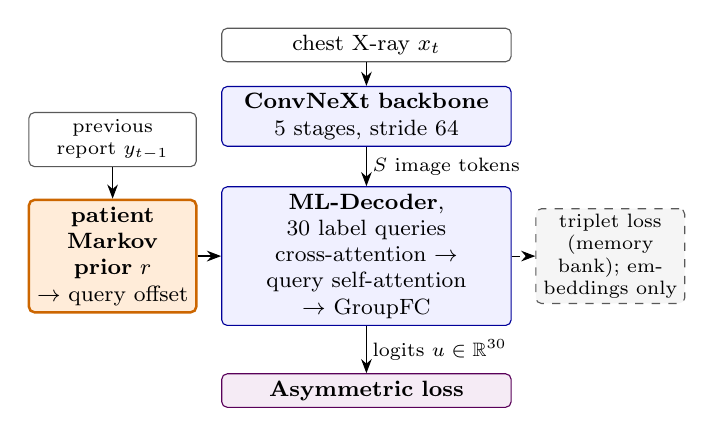
\begin{tikzpicture}[font=\footnotesize, node distance=3mm,
  box/.style={draw=blue!60!black, fill=blue!6, rounded corners=2pt, align=center, text width=3.5cm, inner sep=2.5pt},
  newbox/.style={draw=orange!80!black, fill=orange!15, rounded corners=2pt, align=center, text width=1.95cm, inner sep=2.5pt, line width=0.9pt},
  lossbox/.style={box, draw=violet!70!black, fill=violet!8},
  databox/.style={draw=gray!70!black, fill=white, rounded corners=2pt, align=center, inner sep=2.5pt},
  aux/.style={draw=gray!70!black, dashed, fill=gray!8, rounded corners=2pt, align=center, text width=1.75cm, inner sep=2pt, font=\scriptsize},
  arr/.style={-{Stealth[length=1.8mm]}},
  lab/.style={font=\scriptsize, right, inner sep=2pt}]
\node[databox, text width=3.5cm] (x) {chest X-ray $x_t$};
\node[box, below=of x] (bb) {\textbf{ConvNeXt backbone}\\5 stages, stride 64};
\node[box, below=5mm of bb] (dec) {\textbf{ML-Decoder}, 30 label queries\\cross-attention $\rightarrow$ query self-attention\\$\rightarrow$ GroupFC};
\node[lossbox, below=6mm of dec] (asl) {\textbf{Asymmetric loss}};
\node[aux, right=3mm of dec] (tri) {triplet loss (memory bank); embeddings only};
\node[newbox, left=3mm of dec] (pri) {\textbf{patient Markov prior} $r$\\$\rightarrow$ query offset};
\node[databox, text width=1.95cm, font=\scriptsize, above=4mm of pri] (rep) {previous report $y_{t-1}$};
\draw[arr] (x) -- (bb);
\draw[arr] (bb) -- node[lab]{$S$ image tokens} (dec);
\draw[arr] (dec) -- node[lab]{logits $u \in \mathbb{R}^{30}$} (asl);
\draw[arr, dashed] (dec) -- (tri);
\draw[arr] (rep) -- (pri);
\draw[arr, line width=0.9pt] (pri) -- (dec);
\end{tikzpicture}
\caption{Where the Markov priors enter. The baseline (v3) is the model without the orange box. In the in-network variant (Section~\ref{sec:phprior}), the patient-history Markov prior $r$, computed from the previous report, offsets the ML-Decoder label queries. In the post-prediction variant (Section~\ref{sec:hmm}), the same chain is fused with the probabilities $\sigma(u)$ of a frozen model, together with metadata (Fig.~\ref{fig:hmm}). The label-graph priors of Sections~\ref{sec:smoothing} and~\ref{sec:gating} act on $\sigma(u)$ at inference.}
\label{fig:pipeline}
\end{figure}

\subsection{Label Transition Matrix}
Let $C_{ij}$ be the number of training images labelled with both $i$ and $j$. The co-occurrence Markov chain has transition matrix
\begin{equation}
P_{ij} = \frac{C_{ij}}{\sum_{k \neq i} C_{ik}}, \quad i \neq j, \qquad P_{ii} = 0,
\label{eq:transition}
\end{equation}
so each row is a probability distribution over the labels that accompany label $i$. $P$ is built from the training fold only. Row normalisation has one unavoidable side effect: the Normal row must also sum to one, so $P$ cannot express that Normal excludes every finding.

\subsection{Post-Hoc Random-Walk Smoothing}
\label{sec:smoothing}
Given an image's predicted probabilities $p \in [0,1]^{30}$, let $s = \sum_c p_c$ and $\hat{p} = p / s$. One random-walk step redistributes the normalised mass along $P$, and we blend it with the original prediction,
\begin{equation}
q = (1 - \alpha)\, p + \alpha\, s\, (\hat{p} P),
\label{eq:smoothing}
\end{equation}
where $\alpha$ sets the strength of the prior. Multiplying by $s$ keeps the total mass of $q$ equal to that of $p$.

\subsection{Normal-Gating}
\label{sec:gating}
The Task~1 winner~\cite{b15} suppresses every abnormal class $c \neq 0$ by the predicted probability $p_0$ of the Normal class,
\begin{equation}
p_c \leftarrow p_c\,(1 - p_0)^{\alpha_{ng}}, \qquad \alpha_{ng} = 0.5.
\label{eq:gating}
\end{equation}
This is a hard-exclusivity prior. In our validation labels, Normal co-occurs with an abnormal finding in only 26 of 17,270 images. We also test a reverse gate that suppresses Normal instead, $p_0 \leftarrow p_0\,(1 - \max_{c \neq 0} p_c)^{0.5}$.

\subsection{Patient-History Markov Prior}
\label{sec:phprior}
The patient-history prior uses the order of a patient's studies. We group studies into states, one per patient and date; the state $y_t \in \{0,1\}^{30}$ is the union of the label sets of that date's studies, as read from their reports. For each class, a two-state Markov chain gives the probability that the finding is present at a state, given whether it was present at the patient's previous state:
\begin{equation}
\pi_c(y_{t-1}) = \begin{cases} a_c, & y_{t-1,c} = 1,\\ b_c, & y_{t-1,c} = 0, \end{cases}
\label{eq:chain}
\end{equation}
with $a_c$ and $b_c$ estimated, with Laplace smoothing, from the 24,180 pairs of consecutive states in the training fold. For an image whose patient has a strictly earlier state, we summarise the prior as
\begin{equation}
r = \bigl[\operatorname{logit} \pi_c(y_{t-1}) - \operatorname{logit} \bar\pi_c\bigr]_{c=1}^{30} \oplus 1,
\label{eq:rvec}
\end{equation}
where $\bar\pi_c$ is the training prevalence of class $c$ and the last entry flags that a prior exists; an image without an earlier state gets $r = 0$. We use the prior in two ways.

\textbf{In-network.} The prior offsets the 30 ML-Decoder label queries before they attend to the image:
\begin{equation}
Q_c \leftarrow Q_c + r_c\, u_c + W r, \qquad c = 1, \dots, 30,
\label{eq:qprior}
\end{equation}
where $u \in \mathbb{R}^{30 \times 768}$ and $W \in \mathbb{R}^{768 \times 31}$ start at zero, so training starts exactly from the baseline and an image without a prior always receives a zero offset. During training, each image's prior is set to zero with probability 0.3, so the network also learns to classify without it. Patient identity is used only to find the earlier state; no metadata enter the network.

\textbf{Post-prediction.} Alternatively, the classifier is kept frozen and the chain becomes the transition of a hidden Markov model whose emission is the classifier output (Section~\ref{sec:hmm}). Its simplest calibrated arm (H1) adds $w_h\,[\operatorname{logit} \pi_c(y_{t-1}) - \operatorname{logit} \bar\pi_c]$ to the calibrated logits, with $w_h$ fitted on held-out patients; richer arms add the time gap, patient and study metadata, and cross-class terms to the transition.

\subsection{Post-Prediction Patient HMM}
\label{sec:hmm}
For post-prediction fusion we keep the classifier frozen and place the Markov model after it, so that the network only extracts image evidence and the patient information enters through the prior.

\textbf{Graphical model.} A patient's studies are grouped into states, one per patient and date (Fig.~\ref{fig:hmm}). The state $y_t \in \{0,1\}^{30}$ is the element-wise OR of the label vectors of that date's studies, and $m_t$ is the date's metadata. The model is a hidden Markov model whose emission is the classifier:
\begin{equation}
p(y_{1:T}, x_{1:T}) = p(y_1 \mid m_1) \prod_{t>1} p(y_t \mid y_{t-1}, m_t) \prod_{t} p(x_t \mid y_t).
\label{eq:hmm}
\end{equation}
The emission can come from any classifier that outputs probabilities; we use the ConvNeXt/ML-Decoder models of Section~\ref{sec:setup}, which have no Mixture-of-Experts head.

\begin{figure}[htbp]
\centering
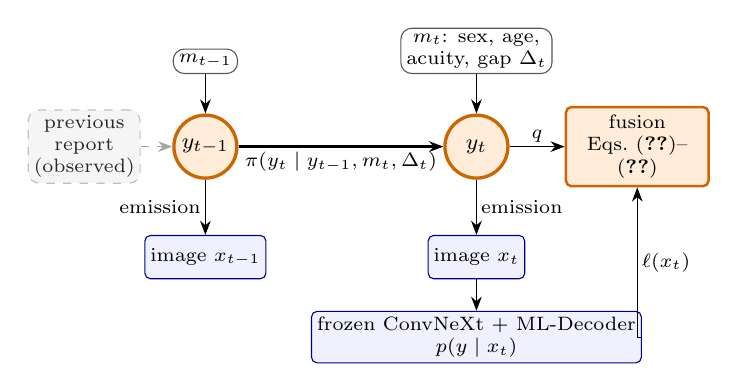
\begin{tikzpicture}[font=\footnotesize,
  st/.style={circle, draw=orange!80!black, fill=orange!15, line width=1.2pt, minimum size=8mm, inner sep=0pt},
  img/.style={draw=blue!60!black, fill=blue!6, rounded corners=2pt, align=center, inner sep=2pt, minimum height=5.5mm, font=\scriptsize},
  meta/.style={draw=gray!70!black, fill=white, rounded corners=4pt, align=center, inner sep=2pt, font=\scriptsize},
  aux/.style={draw=gray!50, dashed, fill=gray!8, rounded corners=4pt, align=center, inner sep=2pt, font=\scriptsize, text=gray!30!black},
  fuse/.style={draw=orange!80!black, fill=orange!15, rounded corners=2pt, align=center, inner sep=3pt, line width=0.9pt, font=\scriptsize},
  arr/.style={-{Stealth[length=1.8mm]}},
  lab/.style={font=\scriptsize, inner sep=1.5pt}]
\node[st] (y0) {$y_{t-1}$};
\node[st, right=26mm of y0] (y1) {$y_t$};
\node[meta, above=5mm of y0] (m0) {$m_{t-1}$};
\node[meta, above=5mm of y1] (m1) {$m_t$: sex, age,\\acuity, gap $\Delta_t$};
\node[aux, left=4mm of y0] (rep) {previous\\report\\(observed)};
\node[img, below=7mm of y0] (x0) {image $x_{t-1}$};
\node[img, below=7mm of y1] (x1) {image $x_t$};
\node[img, below=4mm of x1] (clf) {frozen ConvNeXt + ML-Decoder\\$p(y \mid x_t)$};
\node[fuse, right=7mm of y1, text width=1.6cm] (fz) {fusion\\Eqs.~\eqref{eq:fuse}--\eqref{eq:qw}};
\draw[arr, line width=1.2pt] (y0) -- node[lab, below]{$\pi(y_t \mid y_{t-1}, m_t, \Delta_t)$} (y1);
\draw[arr] (m0) -- (y0);
\draw[arr] (m1) -- (y1);
\draw[arr] (y0) -- node[lab, left]{emission} (x0);
\draw[arr] (y1) -- node[lab, right]{emission} (x1);
\draw[arr, dashed, draw=gray!70] (rep) -- (y0);
\draw[arr] (x1) -- (clf);
\draw[arr] (clf.east) -| node[lab, pos=0.75, right]{$\ell(x_t)$} (fz.south);
\draw[arr] (y1) -- node[lab, above]{$q$} (fz);
\end{tikzpicture}
\caption{The post-prediction patient HMM as a graphical model, with one state per patient and date. Orange circles are the hidden finding states $y_t \in \{0,1\}^{30}$, blue boxes the images and the frozen classifier, white boxes metadata. The transition prior $\pi$ (Eq.~\eqref{eq:trans}) depends on the previous state, the metadata of the current date and the gap $\Delta_t$; a state without an earlier state uses $\pi^{0}(m)$ (Eq.~\eqref{eq:init}). The classifier supplies only the emission (Eq.~\eqref{eq:emission}), and prior and emission are combined after the network. In the observed mode $y_{t-1}$ is read from the previous report (dashed); in the filtered mode it is inferred from $x_{1:t-1}$ by Eqs.~\eqref{eq:predict}--\eqref{eq:update}.}
\label{fig:hmm}
\end{figure}

\textbf{Emission.} The classifier gives posteriors $p_c(x) = P(y_c{=}1 \mid x)$. After a calibration fitted on held-out patients, with a temperature $\tau$ shared by all classes and a per-class intercept $\delta_c$, the posterior is converted into a likelihood ratio by dividing out the training prevalence $\bar\pi_c$:
\begin{equation}
\ell_c(x) = \tau \operatorname{logit} p_c(x) + \delta_c - \operatorname{logit} \bar\pi_c .
\label{eq:emission}
\end{equation}

\textbf{Prior.} The prior factorises over classes, each a logistic model. A state without an earlier state uses $\pi^{0}$; later states use the transition $\pi$:
\begin{align}
\operatorname{logit} \pi^{0}_c(m) &= \alpha^{0}_c + \gamma^{0\top}_c \phi(m), \label{eq:init}\\
\operatorname{logit} \pi_c(y', m, \Delta) &= \alpha_c + \beta_c y'_c + \kappa_c y'_c g + \lambda_c g \nonumber\\
&\quad + \textstyle\sum_{k \neq c} B_{ck}\, y'_k + \gamma_c^{\top} \phi(m), \label{eq:trans}
\end{align}
where $y'$ is the previous state, $g = \log(1 + \Delta)$ for a gap of $\Delta$ days, and $B_{ck}$ is a cross-class temporal edge from class $k$ at the previous state to class $c$ at the current one. The metadata enter as
\begin{equation}
\phi(m) = \bigl[\mathbf{1}_{\mathrm{M}},\ \mathbf{1}_{\mathrm{U}},\ \operatorname{rcs}(\text{age}),\ \mathbf{1}_{\mathrm{AP}},\ \mathbf{1}_{\mathrm{APh}}\bigr],
\label{eq:phi}
\end{equation}
where $\mathbf{1}_{\mathrm{M}}$ and $\mathbf{1}_{\mathrm{U}}$ indicate male and unknown sex, $\operatorname{rcs}$ is a restricted cubic spline of age with knots at the 5th, 35th, 65th and 95th percentiles (three terms), and $\mathbf{1}_{\mathrm{AP}}$ and $\mathbf{1}_{\mathrm{APh}}$ indicate the acuity of the date, an AP or AP horizontal projection against PA or lateral; each column is standardised on the training states. All 30 logistic models are fitted at once, as one batched model in double precision, by L-BFGS on consecutive states of the training fold; $\pi^{0}$ is fitted on the patients' first states. The L2 penalties are chosen by patient-grouped five-fold cross-validated log-loss on the training pairs, and the intercepts $\alpha_c$, $\alpha^0_c$ and the own-state terms $\beta_c$ are not penalised.

\textbf{Fusion.} For a target image $x$ on date $t$,
\begin{align}
z_c &= \tau \operatorname{logit} p_c(x) + \delta_c + w \bigl[\operatorname{logit} q_c - \operatorname{logit} \bar\pi_c\bigr], \label{eq:fuse}\\
(q_c, w) &= \begin{cases}
\bigl(\pi_c(y_{t-1}, m_t, \Delta_t),\ w_h\bigr) & \text{earlier state},\\
\bigl(\pi^{0}_c(m_t),\ w_0\bigr) & \text{otherwise}.
\end{cases} \label{eq:qw}
\end{align}
With $w = 1$ this is Bayes' rule: the prior log-odds plus the emission likelihood ratio of Eq.~\eqref{eq:emission}. We instead fit $w_h$ and $w_0$ on held-out patients, for two reasons: the ASL-trained probabilities are not calibrated posteriors, and the image and the prior can carry the same evidence (a device is both visible in the current image and recorded in the previous report). With $w_h = w_0 = 0$ the model returns the classifier's ranking unchanged.

\textbf{History.} The previous state $y_{t-1}$ can be obtained in two ways (Table~\ref{tab:modes}). In the \emph{observed} mode, it is the label set of the previous report, which a reading radiologist has at hand, and the prior is exactly Eq.~\eqref{eq:trans}. In the \emph{filtered} mode, the previous state is inferred from the patient's earlier images alone by a forward pass with a factorised belief $\mu_t$:
\begin{align}
q_c &= \mu_{t-1,c}\, \sigma\bigl(\eta_c(1, \mu_{t-1})\bigr) \nonumber\\
&\quad + (1 - \mu_{t-1,c})\, \sigma\bigl(\eta_c(0, \mu_{t-1})\bigr), \label{eq:predict}\\
\mu_{t,c} &= \sigma\bigl(\operatorname{logit} q_c + w_e\, \bar\ell_{t,c}\bigr), \label{eq:update}
\end{align}
where $\eta_c(s, \mu)$ is the logit of Eq.~\eqref{eq:trans} with $y'_c = s$ and the other classes at their beliefs, and $\bar\ell_t$ is the mean of Eq.~\eqref{eq:emission} over the images of date $t$. The prediction step is exact when $B = 0$; with cross-class edges it is a mean-field (Boyen--Koller~\cite{b24}) projection. With one-hot beliefs the filtered mode reproduces the observed mode exactly, which our code asserts. At the target date only the target image itself enters; same-date views of other images are not fused, because that would add an unrelated multi-view gain.

\begin{table}[htbp]
\caption{The two history modes of the patient HMM.}
\begin{center}
\footnotesize
\setlength{\tabcolsep}{3pt}
\begin{tabular}{|l|>{\raggedright\arraybackslash}p{2.9cm}|>{\raggedright\arraybackslash}p{3.3cm}|}
\hline
\textbf{Mode} & \textbf{Source of $y_{t-1}$} & \textbf{Prior $q_c$} \\
\hline
observed & labels (0/1) of the previous state's report & $q_c = \pi_c(y_{t-1}, m_t, \Delta_t)$, exact (Eq.~\eqref{eq:trans}) \\
\hline
filtered & belief $\mu_{t-1}$ from a forward pass over all earlier states' images & Eq.~\eqref{eq:predict}, then the update Eq.~\eqref{eq:update}; exact when $B = 0$, mean field otherwise \\
\hline
\end{tabular}
\label{tab:modes}
\end{center}
\end{table}

\textbf{Arms.} The arms add terms in a fixed, pre-specified order (Table~\ref{tab:arms}); H4 is the primary arm. H0 reproduces the late fusion of our earlier study exactly, which our code asserts. Three ablations extend H4.

\begin{table}[htbp]
\caption{Arms of the patient HMM. Each arm adds to the one above it; H4 is the pre-specified primary arm, and H5, H4-acq and H4-F are ablations of it.}
\begin{center}
\footnotesize
\setlength{\tabcolsep}{3pt}
\begin{tabular}{|l|>{\raggedright\arraybackslash}p{6.6cm}|}
\hline
\textbf{Arm} & \textbf{Adds} \\
\hline
E & the emission only ($w_h = w_0 = 0$) \\
H0 & pooled per-class two-state chain, $a_c = P(1 \mid 1)$ and $b_c = P(1 \mid 0)$ with Laplace smoothing; $w_h = 1$, no calibration. Reproduces the late fusion of our earlier study exactly \\
H1 & $+$ calibration ($\tau$, $\delta$) and a cross-fitted $w_h$ \\
H2 & $+$ gap terms $\kappa$, $\lambda$ \\
H3 & $+$ metadata $\phi(m)$ in $\pi$ and $\pi^{0}$; $w_0$ then also changes images without an earlier state \\
\textbf{H4} & $+$ cross-class temporal edges $B_{ck}$ (class $k$ at $t-1$ to class $c$ at $t$) \\
\hline
H5 & $+$ within-state label couplings $J$: a pairwise Markov random field fitted by pseudo-likelihood, applied by damped mean field with a fitted weight $w_J$ \\
H4-acq & $+$ per-state DICOM acquisition fields in $\phi$ (care-setting proxies) \\
H4-F & H4 in the filtered mode \\
\hline
\end{tabular}
\label{tab:arms}
\end{center}
\end{table}


\section{Markov Experiments: Setup}
\label{s:mksetup}\label{sec:setup}
\textbf{Data.} We use the CXR-LT 2026 Task~1 training data: PadChest~\cite{b9} images with 30 report-derived target labels, split into an internal training fold (103,303 images after filtering) and a validation fold (17,270 scored images). Patient identifiers, study identifiers and projections come from the original PadChest metadata.

\textbf{Post-hoc experiments.} Sections~\ref{sec:smoothing} and~\ref{sec:gating} are evaluated on cached validation probabilities with horizontal-flip test-time augmentation (TTA). The base model is our best greedy three-model ensemble of v3 models: two SWA checkpoints (768~px, seed 42; 1024~px, seed 86) and one best-epoch checkpoint (640~px, seed 86). The ensemble is a uniform average of probabilities; its members were chosen by forward selection, adding at each step the model that most raised validation mAP and stopping when the gain fell below $10^{-4}$. Because the members were selected on the fold they are scored on, its mAP of 0.4722 is slightly optimistic; the fixed average of four v3 SWA models scores 0.4699. Neither contains a Markov component. The metric is macro mAP over the 30 classes. No model is retrained.

\textbf{Patient-history prior (in-network).} Each seed (42 and 1024) fine-tunes from the same Stage-1 checkpoint with our final Stage-2 recipe (768~px input, drop-path 0.1, four epochs of an eight-epoch cosine schedule, effective batch size 48, triplet weight $\lambda = 0.1$ and a memory bank of 2,048 embeddings), with the prior of Eq.~\eqref{eq:qprior}, prior dropout 0.3, and a learning rate ten times the base rate ($10^{-3}$ versus $10^{-4}$) for $u$ and $W$. The baselines are the identical runs without the prior. Training images take their earlier state from the training fold only, so no validation label reaches a training input; validation images take it from both folds, as in a hospital archive, and 5,759 of the 17,270 have one. We report the stochastic weight average (SWA) of the EMA weights over the last three epochs, evaluated with horizontal-flip TTA both with the prior and with every prior set to zero (\emph{withheld}), the only condition available on the test set. Because no weight is fitted on validation data, these models are scored on the whole fold.

\textbf{Metadata analysis.} We relate PadChest patient, study and acquisition metadata to the 30 labels on the training fold only (50,604 patients, 75,819 studies). Labels come from the challenge label lists, never from the PadChest report or label columns, and only a whitelist of metadata columns is read, for training and validation images only. Patient and study fields (sex, age at study, pediatric flag, number of earlier states, days since the previous study, study year, study acuity) are counted per study; view and acquisition fields (projection, scanner manufacturer, spatial resolution, exposure, image size and others) are counted per image. For each field and class we compute Cram\'er's V, mutual information, a chi-square test with Benjamini--Hochberg correction, and the log odds ratio of the most extreme level with a patient-clustered bootstrap interval (200 resamples). The tests ignore the clustering of studies within patients, so we rank by effect size. A per-class logistic regression on metadata alone is scored by patient-grouped five-fold cross-validation, with each feature group (patient: sex and age; temporal; view; acquisition) alone and removed in turn. To test whether metadata add to the image model, we fit on the validation fold, for each class, a logistic model of the label on the image logit plus the metadata, fitted on one half of the patients and scored on the other (both directions). We compute mAP within each half, average the two, and compare with the unmodified image probabilities by a paired patient-clustered bootstrap (300 resamples). The image models are the 768~px seed-42 SWA model and the greedy three-model ensemble, both with flip TTA.

\textbf{Longitudinal simulation.} Route (B) is evaluated on the internal folds only, as a simulation of reading with prior studies; no development or test image is ever linked to the PadChest metadata, and only a whitelist of metadata columns is read (dates, projection, sex and birth year, plus acquisition fields for H4-acq), never the report or label columns. The prior is fitted on training-fold states only (74,782 states, 24,180 consecutive pairs). Validation images take their history from both folds, as in a hospital archive: 5,759 of the 17,270 have an earlier state, and the primary subset is the 4,061 of these that are frontal. Calibration and fusion weights are cross-fitted: the validation patients are split into two halves, all parameters are fitted on one half (the weights by macro mAP on the grid $\{0, 0.25, \dots, 1.5\}$) and applied to the other, for three random splits. Because the halves receive different calibrations, AP is computed within each half and averaged; pooling them would mix two scales inside each class ranking. The emissions are the 768~px SWA models at seeds 42 and 1024 and the greedy ensemble, all with flip TTA, and the in-network prior is compared with the emission of the same seed. In the filtered mode, training-fold images have in-sample emissions from the seed-42 model (mAP 0.713 on the training fold), so a filtered history built from training images is optimistic. Differences use a paired patient-clustered bootstrap of 300 resamples on the first split.

\textbf{Validation subsets.} To compare with the test set, we split the validation fold by projection (frontal: PA, AP and AP horizontal; lateral) and by whether the image's patient also appears in the training fold. Scores on a subset are macro mAP over the classes with at least one positive in that subset (28 classes for the frontal, unseen-patient subset). The cached probabilities carry no sample keys, so we rebuilt their row order from the evaluation data-loader schedule; the rebuilt order reproduces all 17,270 stored label rows exactly, and only one arrangement of the four images missing from the shards fits. Differences between two models are tested with a patient-clustered bootstrap of 300 resamples.


\section{Markov Experiments: Results}
\label{s:mkres}

\subsection{Random-Walk Smoothing}
Table~\ref{tab:smoothing} shows that smoothing lowers mAP at every strength, and the loss grows with $\alpha$. At $\alpha = 0.05$ the loss falls mainly on the head classes: the mean change in per-class AP is $-0.0021$ over the ten most frequent classes and $-0.0001$ over the ten rarest.

\begin{table}[htbp]
\caption{Post-hoc random-walk smoothing (Eq.~\eqref{eq:smoothing}) applied to the greedy-3 ensemble of our entropy-gated v3 model (Table~\ref{M-m:tab-entropy}), flip TTA, $n_{val} = 17{,}270$. The first row is that model without any Markov step; its 0.4722 is the entropy-gated model's own score. Every smoothing strength lowers it.}
\begin{center}
\begin{tabular}{|c|c|c|}
\hline
$\boldsymbol{\alpha}$ & \textbf{mAP} & \textbf{$\Delta$ vs base} \\
\hline
0 (entropy-gated v3, no Markov) & 0.4722 & --- \\
\hline
0.02 & 0.4716 & $-0.0006$ \\
\hline
0.05 & 0.4710 & $-0.0012$ \\
\hline
0.10 & 0.4698 & $-0.0024$ \\
\hline
0.20 & 0.4669 & $-0.0053$ \\
\hline
\end{tabular}
\label{tab:smoothing}
\end{center}
\end{table}

AP is a per-class ranking metric. Smoothing moves probability from an image's confident findings to findings that accompany them \emph{on average}, which blurs the per-image evidence the ranking depends on. The ML-Decoder already learns label interactions through its queries, so a fixed co-occurrence prior adds no new information.

\subsection{Normal-Gating}
Normal-gating lowers mAP at every strength (Table~\ref{tab:gating}); at the winner's setting ($\alpha_{ng} \ge 0.5$) 28 of 30 classes get worse (26 at $\alpha_{ng} = 0.25$). The single 1024~px model behaves the same way ($-0.024$ at $\alpha_{ng} = 0.5$). The reverse gate leaves mAP unchanged. The winner trained with a Distribution-Balanced loss~\cite{b23} and class-aware sampling, both of which push abnormal scores up, and used the gate to \emph{``suppress spurious abnormal predictions''}~\cite{b15}. Our Asymmetric-Loss model has no such bias, so the gate only spreads the errors in $p_0$ into every other class's ranking. This comparison uses report-derived labels; the leaderboard uses radiologist labels.

\begin{table}[htbp]
\caption{Normal-gating (Eq.~\eqref{eq:gating}) applied to the greedy-3 ensemble of our entropy-gated v3 model (Table~\ref{M-m:tab-entropy}), flip TTA. The first row is that model without any Markov step (the entropy-gated model's own score); every gate lowers it or leaves it unchanged.}
\begin{center}
\begin{tabular}{|l|c|c|}
\hline
\textbf{Variant} & \textbf{mAP} & \textbf{$\Delta$} \\
\hline
entropy-gated v3, no Markov & 0.4722 & --- \\
\hline
gate, $\alpha_{ng} = 0.25$ & 0.4619 & $-0.0103$ \\
\hline
gate, $\alpha_{ng} = 0.5$ (winner's setting) & 0.4483 & $-0.0239$ \\
\hline
gate, $\alpha_{ng} = 1.0$ & 0.4264 & $-0.0459$ \\
\hline
reverse gate on Normal & 0.4722 & $\pm 0.0000$ \\
\hline
\end{tabular}
\label{tab:gating}
\end{center}
\end{table}

\subsection{Patient-History Markov Prior (In-Network)}
\label{sec:phres}
Table~\ref{tab:phprior} compares each in-network model with its baseline. With the patient-history prior, mAP rises by $+0.019$ at both seeds (0.4650 to 0.4839 and 0.4626 to 0.4820), and the training-log SWA scores without TTA give the same picture (0.4600 to 0.4807 and 0.4582 to 0.4786). Almost all of the gain is on the 5,759 images with an earlier state (0.4894 to 0.5276 at seed 42), 98.6\% of which belong to patients also in the training fold; on the frontal ones, the paired difference is $+0.0270$ (95\% CI $+0.0081$ to $+0.0497$) at seed 42 and $+0.0380$ ($+0.0265$ to $+0.0547$) at seed 1024. On images without an earlier state, where the offset is zero by construction, the network trained with the prior scores 0.4562 against 0.4529 at seed 42. On the frontal images with an earlier state, the gain reaches all 3 head and all 20 medium classes at seed 42 (mean $\Delta$AP $+0.0175$ and $+0.0360$) and 5 of the 7 tail classes ($+0.0055$; $+0.0546$, 6 of 7, at seed 1024). With the prior withheld, mAP is 0.4624 against 0.4650 at seed 42 (paired $-0.0026$, $-0.0109$ to $+0.0075$) and 0.4663 against 0.4626 at seed 1024 ($+0.0037$, $-0.0029$ to $+0.0106$): without history, the network is no better than the baseline. A two-seed ensemble scores 0.4867 with the prior and 0.4693 with it withheld, against 0.4659 for the two baseline models. Table~\ref{tab:hmm} scores the same models within patient halves, to match the cross-fitted HMM, so its in-network rows differ slightly from these.

\begin{table}[htbp]
\caption{Patient-history Markov prior fed into the network (in-network), against the identical model without it (v3): internal validation, flip TTA, SWA weights. Withheld: the same network with every prior set to zero, the only condition available on the test set. Earlier: images whose patient has an earlier state (5,759); frontal earlier: the frontal ones among them (4,061); none: images without an earlier state (11,511).}
\begin{center}
\footnotesize
\setlength{\tabcolsep}{4pt}
\begin{tabular}{|l|l|c|c|c|c|}
\hline
\textbf{Seed} & \textbf{Model} & \textbf{All} & \textbf{Earlier} & \textbf{Frontal earlier} & \textbf{None} \\
\hline
42 & v3 & 0.4650 & 0.4894 & 0.4909 & 0.4529 \\
 & + prior & \textbf{0.4839} & \textbf{0.5276} & \textbf{0.5179} & \textbf{0.4562} \\
 & withheld & 0.4624 & 0.4811 & 0.4783 & \textbf{0.4562} \\
\hline
1024 & v3 & 0.4626 & 0.4807 & 0.4791 & 0.4534 \\
 & + prior & \textbf{0.4820} & \textbf{0.5265} & \textbf{0.5171} & \textbf{0.4548} \\
 & withheld & 0.4663 & 0.4830 & 0.4838 & \textbf{0.4548} \\
\hline
\end{tabular}
\label{tab:phprior}
\end{center}
\end{table}

\subsection{Longitudinal Markov Model}
\label{sec:hmmres}
Locally, the longitudinal structure exists. In the PadChest metadata, 13,198 of 50,604 training patients have at least two studies, covering 50.1\% of training images; in the validation fold, 1,548 of 14,501 patients do, covering 21.6\% of images. At test time, however, there is nothing to condition on. The challenge organisers state that \emph{``because PadChest-GR is derived from PadChest, we performed both patient-level and study-level de-duplication to prevent leakage''} and that \emph{``patient identifiers and hidden evaluation labels were not released to participants''}~\cite{b14}. Test patients therefore have no history in the training data. Test images remain linkable in principle to the public PadChest metadata, but participants must follow \emph{``the applicable data-use restrictions, including research-only use, no redistribution, and no attempts to re-identify individual patients''}~\cite{b14}, so building a history this way would breach the terms. We did not attempt it. A longitudinal model is only meaningful in a deployment study with genuine prior studies, the setting of the temporal work in Section~II, which targets progression labels rather than Task~1's static findings.

We nevertheless measure what such a model would do, as a simulation on the internal folds (Section~\ref{sec:hmm}); the leaderboard effect is 0 by construction. Table~\ref{tab:hmm} gives the results, and every difference is relative to the unmodified emission E.

\textbf{Main result.} The primary arm H4 raises mAP on validation images that have an earlier state and are frontal (the primary subset, $n = 4{,}061$) by $+0.0375$ (95\% CI $+0.0228$ to $+0.0513$) with the 768~px seed-42 model and by $+0.0424$ ($+0.0279$ to $+0.0592$) with the seed-1024 model; the three-model ensemble gives $+0.0364$ ($+0.0209$ to $+0.0517$). On the primary subset, mAP goes from 0.502 to 0.541 for seed 42 (mean over three splits). On images with an earlier state, the gain is largest for medium and tail classes ($+0.044$ and $+0.046$ against $+0.013$ for head classes at seed 42, with the CXR-LT frequency groups of 3 head, 20 medium and 7 tail classes), as expected if it comes from findings that persist between visits. Calibration also repairs the probabilities: mECE falls from 0.135 to 0.007.

\textbf{Post-prediction versus in-network.} The paired difference between H4 and the network that is fed the same prior (Section~\ref{sec:phprior}) is $+0.0021$ ($-0.0155$ to $+0.0197$) at seed 42 and $-0.0022$ ($-0.0204$ to $+0.0158$) at seed 1024 on the primary subset, and $-0.0037$ and $-0.0022$ on the full validation fold; every interval includes 0. A model that is retrained with the prior therefore gains nothing over fusing the prior after the classifier, which needs no retraining. Evaluated with its prior withheld, the only condition possible on the test set, the in-network model is no better than E ($-0.0027$ and $+0.0004$ on the full fold).

\textbf{The simplest arm is best.} Adding terms to the chain does not help (Table~\ref{tab:hmm}). H1, which only adds the calibration and a fitted weight $w_h$ to the pooled chain, has the highest mAP on every subset with a prior, at all three emissions (primary subset: 0.5511 against 0.5411 for H4 at seed 42). The gap (H2), metadata (H3), cross-class edges (H4), a within-state random field (H5) and acquisition fields (H4-acq) each add nothing, although the held-out transition prior improves with each of them (macro AUROC 0.66, 0.76, 0.80 and 0.81 for the table, gap, metadata and cross-class models; log-loss 0.1513 to 0.1370). The reason is the one given in Section~\ref{sec:metaeda}: metadata are redundant with the image, and the image already shows what the prior would add. Without the calibration (H0, which reproduces the late fusion of our earlier study), the gain is smaller ($+0.0354$ and $+0.0425$ on the primary subset) and the full-fold change is not significant. The H1 comparisons with the in-network prior are exploratory: $+0.0124$ ($-0.0076$ to $+0.0348$) at seed 42 and $+0.0081$ ($-0.0126$ to $+0.0285$) at seed 1024 on the primary subset.

\textbf{Filtered mode.} Most of the gain needs the previous report. When the previous state is inferred from the patient's earlier images instead of read from the report (H4-F, seed 42), the primary-subset gain falls from $+0.0375$ to $+0.0092$ ($-0.0013$ to $+0.0181$), about a quarter. On the 248 images whose history is entirely out-of-sample it is $+0.0043$ ($-0.0098$ to $+0.0187$). The filtered history of training images uses in-sample emissions (training mAP 0.713 against about 0.465 on validation), so this figure is if anything optimistic. A model that copies the previous report would give the same pattern, and so would genuine persistence of findings; we cannot separate the two with report-derived labels. H4-F is clearly below the in-network prior on the primary subset ($-0.0265$, $-0.0467$ to $-0.0063$, exploratory).

\textbf{Ablations.} The random field (H5) selected its weight $w_J = 0$ in every fold, so H5 equals H4 to four decimals. The strongest within-state couplings it learned are among Normal and pleural effusion ($-1.51$), cardiomegaly ($-1.40$) and Support Devices ($-1.31$), and between Support Devices and central venous catheters ($+1.46$): label correlations that the ML-Decoder head already uses. Acquisition fields (H4-acq) leave the primary-subset gain unchanged ($+0.0377$ against $+0.0375$ at seed 42; $+0.0431$ against $+0.0424$ at seed 1024), although they lower the prior's held-out log-loss from 0.1370 to 0.1346 and raise its AUROC from 0.813 to 0.836. The largest learned cross-class edges are negative from Normal or a sternotomy to a new finding in the next study ($-0.86$ for sternotomy to Normal, $-0.85$ for Normal to pleural effusion).

\textbf{Guards and copy check.} On images with no earlier state, H4 is slightly worse than E at seed 42 ($-0.0009$, $-0.0018$ to $-0.0001$) and neutral at seed 1024 ($-0.0005$, $-0.0015$ to $+0.0005$); H1 leaves these images unchanged. A copy check on findings that are new relative to the previous report (28 classes) shows a small drop in AP for H4 (0.3678 to 0.3621 at seed 42, 0.3647 to 0.3615 at seed 1024; no interval computed). Thus the gain is not bought on new findings, but the prior does not help them either, and the H4 guards are met only approximately. On patients unseen in training, H4 changes mAP by $-0.0053$ ($-0.0151$ to $-0.0006$) at seed 42. Why metadata add nothing is shown in Section~\ref{sec:metaeda}.

\begin{table*}[htbp]
\caption{Post-prediction patient HMM on the internal validation fold: change in macro mAP relative to the emission E (the frozen entropy-gated v3 768~px SWA model with flip TTA, no Markov component; the E row gives absolute mAP). Primary = frontal images with an earlier state ($n = 4{,}061$); full = 17,270 images; no\_prior = 11,511 images without an earlier state. mAP is computed within each of two patient halves (calibration and fusion weights are fitted on one half and applied to the other) and averaged, over three random splits. Each entry is the mean difference with a 95\% CI from a paired patient-clustered bootstrap (300 resamples) on the first split. Entries marked $^\dagger$ (H2, H5) have no bootstrap: they are differences of the three-split mean mAP and are not comparable to the other entries at the 0.001 level. H4-F (image-only history) was run for seed 42 only; In-network and Withheld are the network fed the prior (Section~\ref{sec:phprior}), evaluated with and without it. This is an internal longitudinal simulation with report-derived history; its leaderboard effect is 0. Results for the three-model ensemble are given in the text.}
\begin{center}
\footnotesize
\setlength{\tabcolsep}{3pt}
\begin{tabular}{|l|c|c|c|c|c|c|}
\hline
 & \multicolumn{3}{c|}{\textbf{Seed 42 (768~px)}} & \multicolumn{3}{c|}{\textbf{Seed 1024 (768~px)}} \\
\textbf{Arm} & full & primary & no\_prior & full & primary & no\_prior \\
\hline
E (v3, abs.\ mAP) & 0.4652 & 0.5020 & 0.4543 & 0.4635 & 0.4937 & 0.4551 \\
\hline
H0 & \shortstack{+0.0090\\{[$-$0.0033,+0.0242]}} & \shortstack{+0.0354\\{[+0.0150,+0.0583]}} & 0 (identical) & \shortstack{+0.0115\\{[$-$0.0003,+0.0274]}} & \shortstack{+0.0425\\{[+0.0222,+0.0669]}} & 0 (identical) \\
H1 & \shortstack{+0.0222\\{[+0.0135,+0.0353]}} & \shortstack{+0.0477\\{[+0.0298,+0.0664]}} & 0 (identical) & \shortstack{+0.0259\\{[+0.0165,+0.0396]}} & \shortstack{+0.0527\\{[+0.0346,+0.0752]}} & 0 (identical) \\
H2 & +0.0197$^\dagger$ & +0.0460$^\dagger$ & 0$^\dagger$ & +0.0202$^\dagger$ & +0.0521$^\dagger$ & 0$^\dagger$ \\
H3 & \shortstack{+0.0160\\{[+0.0093,+0.0239]}} & \shortstack{+0.0378\\{[+0.0226,+0.0516]}} & \shortstack{$-$0.0009\\{[$-$0.0018,$-$0.0001]}} & \shortstack{+0.0167\\{[+0.0101,+0.0250]}} & \shortstack{+0.0435\\{[+0.0290,+0.0612]}} & \shortstack{$-$0.0005\\{[$-$0.0015,+0.0005]}} \\
H4 & \shortstack{+0.0152\\{[+0.0089,+0.0226]}} & \shortstack{+0.0375\\{[+0.0228,+0.0513]}} & \shortstack{$-$0.0009\\{[$-$0.0018,$-$0.0001]}} & \shortstack{+0.0158\\{[+0.0090,+0.0245]}} & \shortstack{+0.0424\\{[+0.0279,+0.0592]}} & \shortstack{$-$0.0005\\{[$-$0.0015,+0.0005]}} \\
H5 & +0.0160$^\dagger$ & +0.0390$^\dagger$ & $-$0.0003$^\dagger$ & +0.0168$^\dagger$ & +0.0459$^\dagger$ & $-$0.0002$^\dagger$ \\
H4-acq & \shortstack{+0.0174\\{[+0.0111,+0.0247]}} & \shortstack{+0.0377\\{[+0.0230,+0.0515]}} & \shortstack{$-$0.0001\\{[$-$0.0026,+0.0023]}} & \shortstack{+0.0177\\{[+0.0117,+0.0249]}} & \shortstack{+0.0431\\{[+0.0287,+0.0599]}} & \shortstack{+0.0011\\{[$-$0.0025,+0.0045]}} \\
H4-F & \shortstack{+0.0032\\{[$-$0.0016,+0.0083]}} & \shortstack{+0.0092\\{[$-$0.0013,+0.0181]}} & \shortstack{$-$0.0009\\{[$-$0.0018,$-$0.0001]}} & \multicolumn{3}{c|}{not run} \\
In-network & \shortstack{+0.0191\\{[+0.0129,+0.0257]}} & \shortstack{+0.0339\\{[+0.0152,+0.0554]}} & \shortstack{+0.0014\\{[$-$0.0045,+0.0130]}} & \shortstack{+0.0185\\{[+0.0106,+0.0246]}} & \shortstack{+0.0436\\{[+0.0254,+0.0632]}} & \shortstack{+0.0002\\{[$-$0.0058,+0.0062]}} \\
Withheld & \shortstack{$-$0.0027\\{[$-$0.0092,+0.0047]}} & \shortstack{$-$0.0071\\{[$-$0.0197,+0.0013]}} & \shortstack{+0.0014\\{[$-$0.0045,+0.0130]}} & \shortstack{+0.0004\\{[$-$0.0045,+0.0049]}} & \shortstack{0.0000\\{[$-$0.0074,+0.0091]}} & \shortstack{+0.0002\\{[$-$0.0058,+0.0062]}} \\
\hline
\end{tabular}
\label{tab:hmm}
\end{center}
\end{table*}

\subsection{Patient Metadata and Findings}
\label{sec:metaeda}
\textbf{Associations.} Many fields are associated with the labels (Fig.~\ref{fig:assoc}). The strongest are the acuity of the study (maximum Cram\'er's $V$ 0.528), the projection (0.504), age (0.447) and the time since the previous study (0.447), followed by scanner resolution and exposure fields ($V$ up to 0.406). Sex is weak (maximum $V$ 0.133). The devices are tied to the care setting: Support Devices and central venous catheters occur far more often in portable AP-horizontal studies (log odds ratio $+2.95$ and $+3.52$) and after short gaps. Age drives the other findings (Fig.~\ref{fig:age}): Normal falls from about 70\% of studies below 40 years to about 10\% above 90, while cardiomegaly, aortic elongation, aortic atheromatosis and pleural effusion rise steeply. The single-feature AUROC of age is 0.816 for aortic atheromatosis and 0.776 for aortic elongation. The associations of the tail classes are weak and rest on few positives.

\textbf{Metadata alone.} Metadata predict the labels well above chance. Held-out macro AUROC is 0.760 (chance 0.5) and macro AP is 0.142 (prevalence 0.050); the best classes are central venous catheter (AUROC 0.93) and Support Devices (0.90), and the worst are azygos lobe (0.61) and hypoexpansion (0.64) (Fig.~\ref{fig:auroc}, Table~\ref{tab:metaonly}). Removing the patient fields costs the most (macro AUROC $0.760 \to 0.691$). The acquisition fields rank second, but they identify the scanner and care setting, such as portable AP-supine units, and not patient biology. The AUROCs of the tail classes rest on a handful of positives and are unstable.

\begin{table}[htbp]
\caption{Metadata-only logistic model, patient-grouped five-fold cross-validation on the training fold. Macro average over the 30 classes. Chance: AUROC 0.5, AP 0.050 (mean prevalence).}
\begin{center}
\begin{tabular}{|l|c|c|}
\hline
\textbf{Features} & \textbf{AUROC} & \textbf{AP} \\
\hline
All groups & 0.760 & 0.142 \\
\hline
Patient only & 0.654 & 0.088 \\
\hline
Temporal only & 0.589 & 0.090 \\
\hline
View only & 0.589 & 0.082 \\
\hline
Acquisition only & 0.659 & 0.091 \\
\hline
All $-$ patient & 0.691 & 0.116 \\
\hline
All $-$ temporal & 0.752 & 0.130 \\
\hline
All $-$ view & 0.753 & 0.139 \\
\hline
All $-$ acquisition & 0.729 & 0.133 \\
\hline
\end{tabular}
\label{tab:metaonly}
\end{center}
\end{table}

\textbf{Metadata add nothing to the image.} Stacking metadata on the image logit lowers mAP in every cell (Table~\ref{tab:incr}). On all validation images, the patient fields change mAP by $-0.0026$ (seed 42) and $-0.0049$ (ensemble), and all three groups together by $-0.0095$ and $-0.0123$. On frontal images the changes are similar. The 95\% intervals exclude zero in 15 of 16 cells. This is not a calibration artefact: refitting only a per-class slope and intercept changes mAP by $0.0000$ (seed 42) and $-0.0003$ (ensemble). The image already shows devices, age-related aortic change and the AP-supine geometry, so the metadata add only noise.

\begin{table*}[htbp]
\caption{Change in validation mAP when metadata are stacked on the image logit (cross-fitted on patient halves; 95\% patient-clustered bootstrap interval in brackets). Base: mAP of the entropy-gated v3 image model alone (no Markov, no metadata), averaged over the two halves. s42: 768~px seed-42 SWA model; ens: greedy three-model ensemble; both with flip TTA.}
\begin{center}
\footnotesize
\setlength{\tabcolsep}{2.1pt}
\begin{tabular}{|l|l|c|c|c|c|c|}
\hline
\textbf{Model} & \textbf{Images} & \textbf{Base} & \textbf{+ patient} & \textbf{+ view} & \textbf{+ acquisition} & \textbf{+ all three} \\
\hline
s42 & all & 0.4687 & $-0.0026$ [$-0.0047$, $-0.0004$] & $-0.0036$ [$-0.0075$, $-0.0008$] & $-0.0048$ [$-0.0079$, $-0.0018$] & $-0.0095$ [$-0.0138$, $-0.0056$] \\
\hline
s42 & frontal & 0.4940 & $-0.0028$ [$-0.0050$, $-0.0010$] & $-0.0032$ [$-0.0081$, $+0.0022$] & $-0.0063$ [$-0.0120$, $-0.0018$] & $-0.0106$ [$-0.0174$, $-0.0049$] \\
\hline
ens & all & 0.4785 & $-0.0049$ [$-0.0083$, $-0.0023$] & $-0.0047$ [$-0.0089$, $-0.0019$] & $-0.0069$ [$-0.0110$, $-0.0034$] & $-0.0123$ [$-0.0181$, $-0.0076$] \\
\hline
ens & frontal & 0.5062 & $-0.0060$ [$-0.0153$, $-0.0012$] & $-0.0044$ [$-0.0087$, $-0.0010$] & $-0.0091$ [$-0.0181$, $-0.0031$] & $-0.0158$ [$-0.0264$, $-0.0067$] \\
\hline
\end{tabular}
\label{tab:incr}
\end{center}
\end{table*}

\textbf{Transitions depend on acuity.} In consecutive studies of the same patient (24,180 pairs from the training fold), the chance that a finding persists depends on the acuity of the later study (Fig.~\ref{fig:persist}). Devices and catheters persist more after an AP study: Support Devices 0.578 for PA or lateral studies against 0.834 for AP-horizontal, and central venous catheter 0.269 against 0.812. Normal persists less: 0.676 against 0.258. Sex changes mean persistence by less than 0.01 (0.468 for women, 0.459 for men). The AP cells are small and the per-class values are noisy.

\textbf{Consequence.} Metadata are informative about the findings but redundant with the image. In a longitudinal model they should therefore enter, if at all, through the transition between studies, where acuity and the time gap change persistence, and not as a per-image prior. The labels are derived from reports, so some associations reflect reporting habits. Our validation fold is not patient-disjoint (Section~\ref{sec:audit}). No metadata or history exist for the leaderboard test images and joining them to PadChest is not permitted, so none of these results can change the leaderboard score: the effect there is zero by construction.

\begin{figure*}[htbp]
\centering
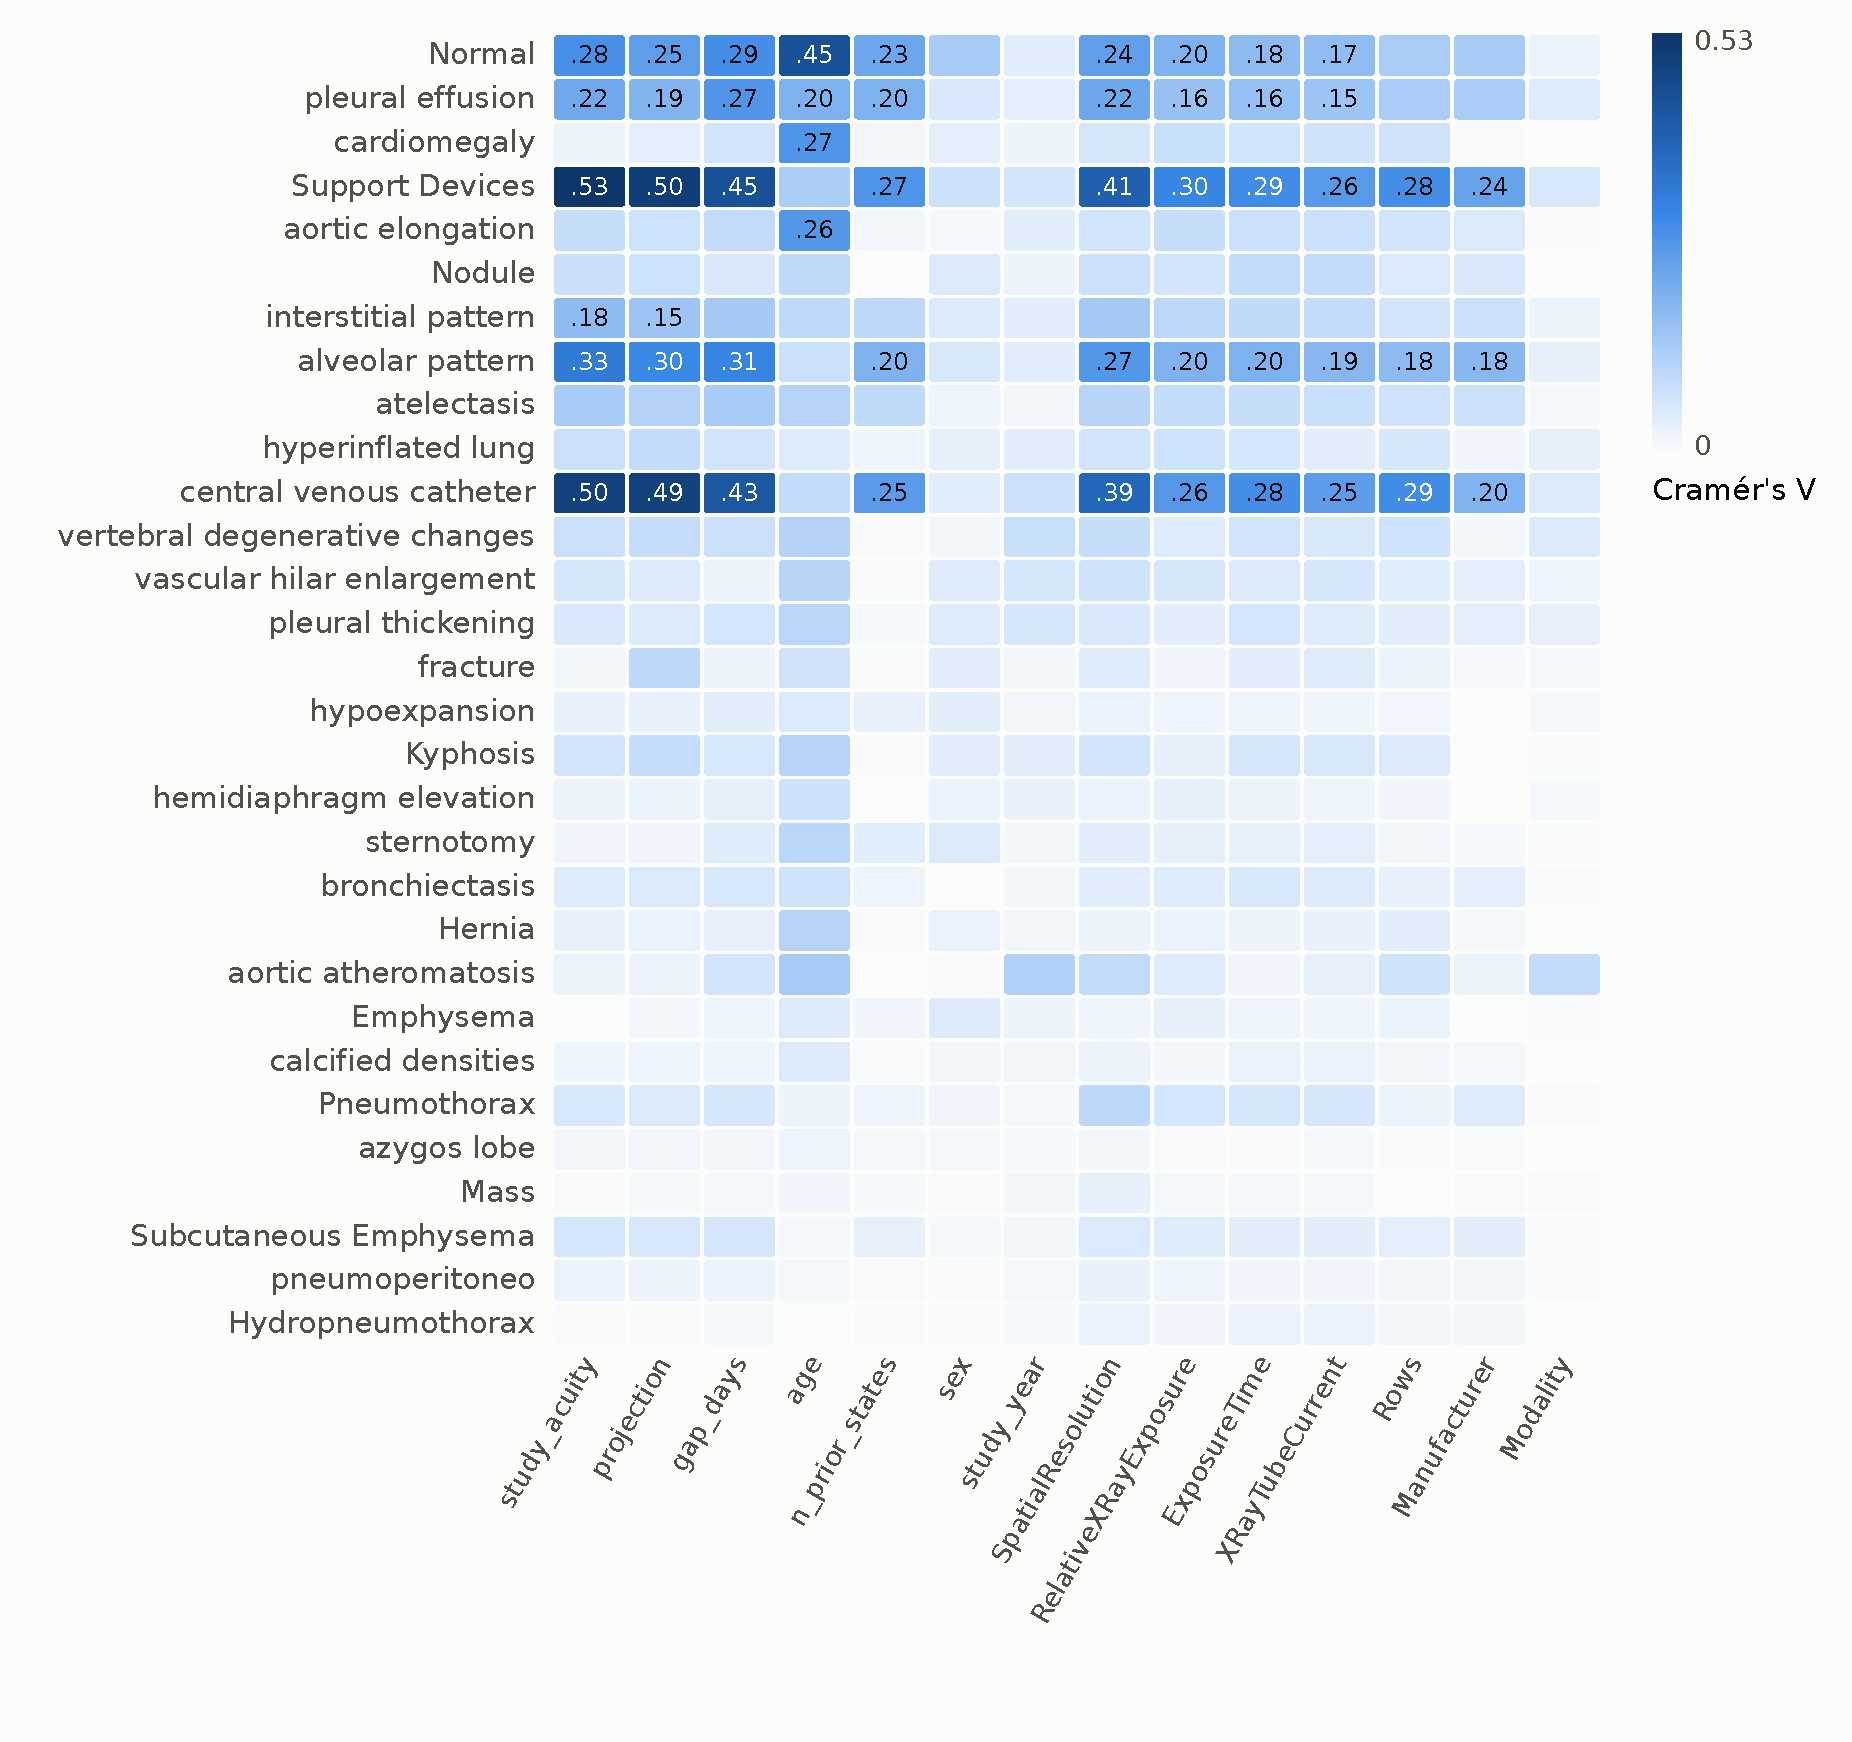
\includegraphics[width=\textwidth]{figures/assoc_heatmap.pdf}
\caption{Association between metadata fields (columns) and the 30 labels (rows, ordered by training prevalence, most frequent at the top) on the training fold. Colour is Cram\'er's $V$ from white (0) to dark blue (0.53); values of 0.15 and above are printed. The study-level fields are acuity, projection, time gap, age, number of earlier studies, sex and year; the remaining columns are acquisition fields (scanner resolution, relative exposure, exposure time, tube current, image rows, manufacturer, modality).}
\label{fig:assoc}
\end{figure*}

\begin{figure*}[htbp]
\centering
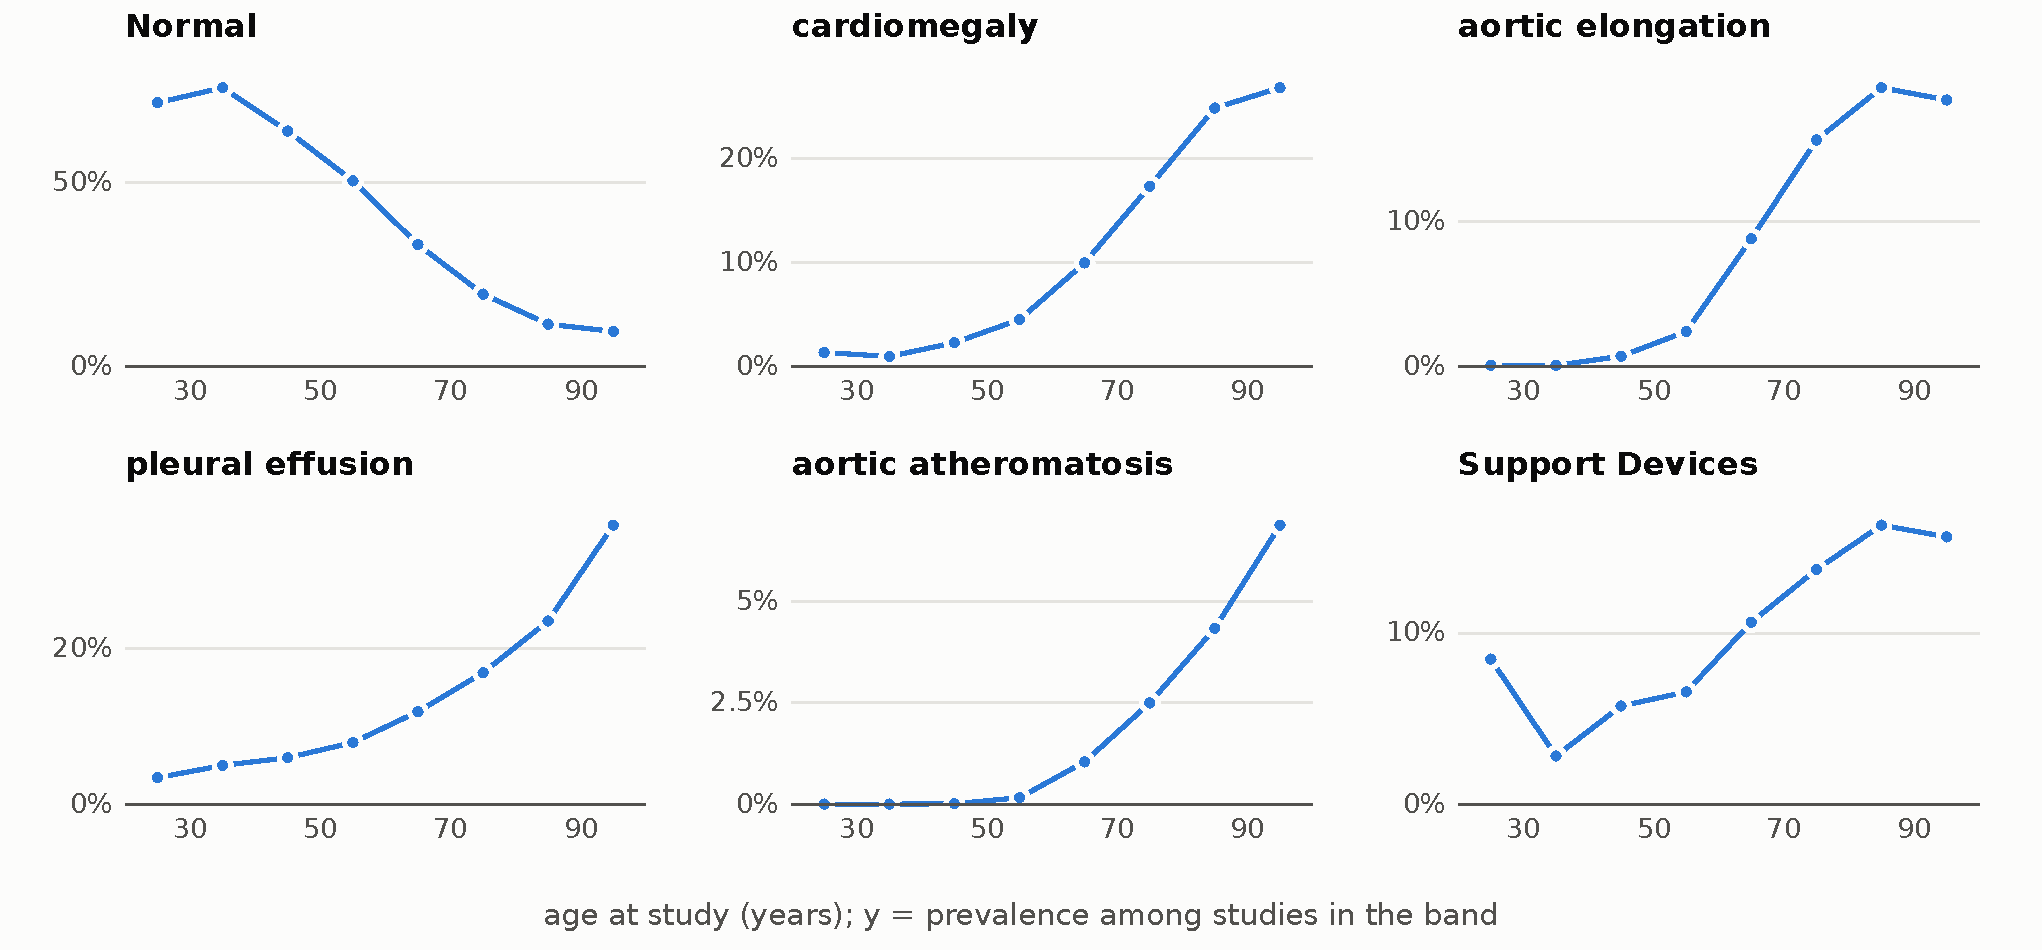
\includegraphics[width=\textwidth]{figures/age_prevalence.pdf}
\caption{Prevalence of six labels by age at study, for the six classes most associated with age. Each point is a 10-year age band of training studies; the vertical axis is the share of studies in the band with the finding. The scales differ between panels.}
\label{fig:age}
\end{figure*}

\begin{figure}[htbp]
\centering
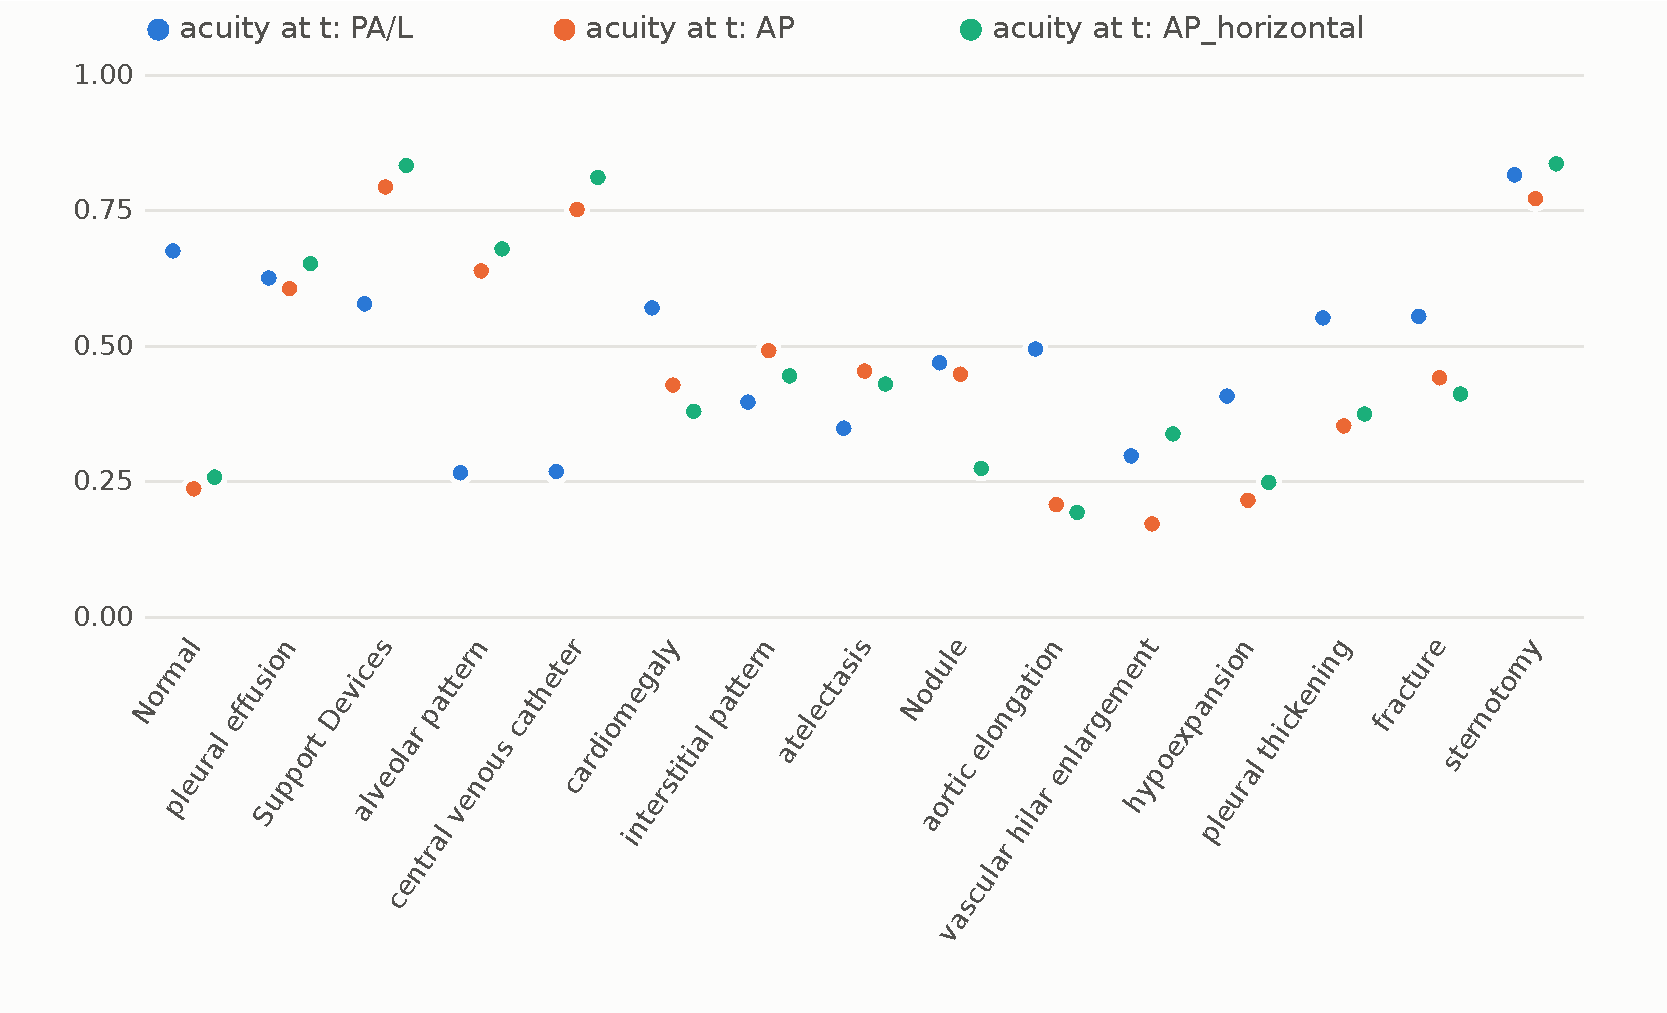
\includegraphics[width=\columnwidth]{figures/persistence_by_acuity.pdf}
\caption{Persistence of findings by the acuity of the later study: the probability that a finding is present at study $t$ given that it was present at study $t-1$ of the same patient (vertical axis), for 15 classes (horizontal axis). Colours give the acuity of study $t$: PA or lateral (blue), AP (orange), AP horizontal (green).}
\label{fig:persist}
\end{figure}

\begin{figure}[htbp]
\centering
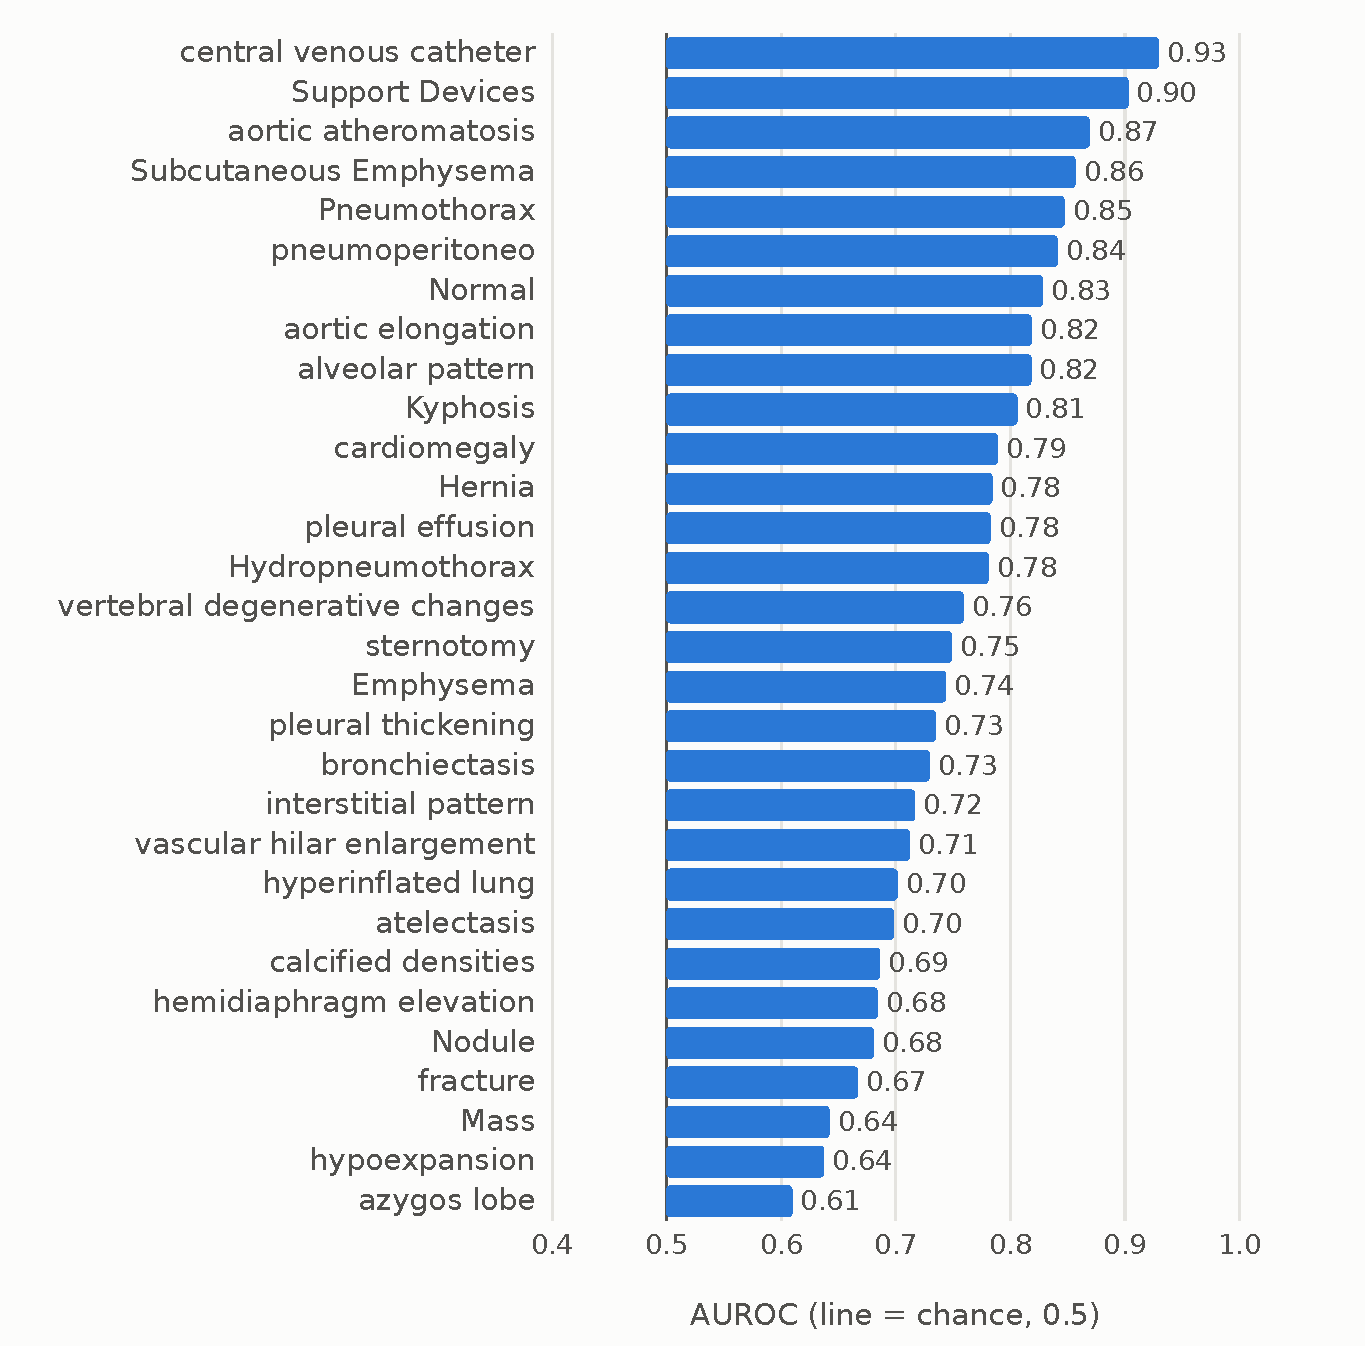
\includegraphics[width=\columnwidth]{figures/metadata_only_auroc.pdf}
\caption{Held-out AUROC of a logistic model that uses metadata only, for each of the 30 classes, sorted from highest to lowest (patient-grouped five-fold cross-validation, training fold). The vertical line marks chance (0.5).}
\label{fig:auroc}
\end{figure}

\subsection{Internal Validation versus the Test Set}
\label{sec:audit}
Checking route (B) required patient identifiers for our own folds, which revealed that our internal validation fold differs from the test set in three ways. The Task~1 test set consists of 3,020 frontal PadChest-GR images (1,620 development, 1,400 test) that each contain at least one target finding, labelled by radiologists and de-duplicated by patient against training~\cite{b14}. Our validation fold, in contrast:
\begin{itemize}
\item \textbf{is not patient-disjoint}: it shares 10,978 patients with the training fold, and 77.0\% of validation images belong to a patient who also appears in training;
\item \textbf{contains lateral views}: 5,234 of 17,270 images;
\item \textbf{uses report-derived labels} rather than radiologist labels.
\end{itemize}

\begin{table*}[htbp]
\caption{Macro mAP (flip TTA) of the entropy-gated v3 models (no Markov component) on subsets of the internal validation fold. These are baseline models, not results of the Markov methods. Seen and unseen refer to whether the image's patient appears in the training fold. The frontal, unseen-patient subset is the closest local proxy for the test set. Each subset is scored over the classes with at least one positive in it.}
\begin{center}
\begin{tabular}{|l|c|c|c|c|c|}
\hline
\textbf{Model} & \textbf{All} & \textbf{Frontal} & \textbf{Lateral} & \textbf{Frontal, seen} & \textbf{Frontal, unseen} \\
 & (17,270) & (11,973) & (5,234) & (8,401) & (3,572) \\
\hline
Greedy-3 v3 ensemble & 0.4722 & 0.4968 & 0.4058 & 0.5025 & 0.4752 \\
\hline
1024~px, SWA (seed 86) & 0.4645 & 0.4892 & 0.3954 & 0.4930 & 0.4719 \\
\hline
768~px, SWA (seed 42) & 0.4650 & 0.4875 & 0.3988 & 0.4945 & 0.4706 \\
\hline
896~px, SWA (seed 86) & 0.4578 & 0.4804 & 0.3927 & 0.4838 & 0.4702 \\
\hline
768~px, resolution sweep (seed 86) & 0.4570 & 0.4785 & 0.3894 & 0.4837 & 0.4642 \\
\hline
640~px, resolution sweep (seed 86) & 0.4485 & 0.4717 & 0.3918 & 0.4801 & 0.4514 \\
\hline
512~px, seed sweep (seed 1024) & 0.4480 & 0.4697 & 0.3873 & 0.4750 & 0.4649 \\
\hline
512~px, drop-path 0.1 (seed 86) & 0.4429 & 0.4641 & 0.3838 & 0.4694 & 0.4644 \\
\hline
\end{tabular}
\label{tab:subsets}
\end{center}
\end{table*}

Table~\ref{tab:subsets} scores eight models on each subset. The SWA rows use our final recipe; the other rows are best-epoch checkpoints from earlier sweeps. For the 1024~px SWA model minus the 512~px seed-1024 model, the patient-clustered bootstrap gives $+0.0196$ [$+0.0047$, $+0.0358$] on frontal, seen-patient images and $+0.0074$ [$-0.0200$, $+0.0269$] on frontal, unseen-patient images. Four observations follow.
\begin{enumerate}
\item \textbf{Lateral views lower the headline number.} On frontal images, the view the test set uses, the v3 ensemble scores 0.4968; the full-fold 0.4722 includes laterals at 0.4058.
\item \textbf{The resolution gain is not established on unseen patients.} The 1024-versus-512~px gain is $+0.020$ with an interval that excludes zero on seen patients, but $+0.007$ with an interval that includes zero on unseen patients. The ordering of the resolutions holds only loosely there, and the 640~px model falls below the 512~px one.
\item \textbf{The seen/unseen gap (0.5025 versus 0.4752) is not all memorisation.} Unseen patients have a different case mix: Normal prevalence 0.58 versus 0.35, 1.27 versus 1.57 labels per image, and 90\% versus 63\% frontal. Only a patient-disjoint re-split with matched case mix can separate the two effects.
\item \textbf{The audit is consistent with the known offset} between our internal and leaderboard scores (Stage~1: 0.385 internal, 0.505 on the development leaderboard). The test set is frontal only, and every test image has at least one finding.
\end{enumerate}


\section{Discussion of the Markov Results}
\label{s:disc}
\textbf{Where the 0.47 comes from.} The 0.4722 in Tables~\ref{tab:smoothing}, \ref{tab:gating} and~\ref{tab:subsets} is the score of our entropy-gated v3 ensemble (Table~\ref{M-m:tab-entropy}), used unchanged as the baseline; both label-graph priors score at or below it, and the patient-history prior is compared with the same single model without it (Table~\ref{tab:phprior}), not with this ensemble, which sees no history. Its rise from the 0.414 of the original implementation came from correcting that implementation and scaling the recipe (Section~\ref{s:v3}), not from label priors, and no run switches off the entropy gate or the triplet term, so these figures do not show how much of the 0.47 the gate itself contributes.

\textbf{Why label priors do not help here.} ML-Decoder's query self-attention is itself a row-stochastic $30 \times 30$ mixing over labels. It is recomputed for every image, operates on 768-dimensional label embeddings, and is repeated over 8 heads in each of 2 blocks. A label-graph prior instead applies one global matrix to the probabilities. For a ranking metric, a global matrix can only move scores in the same direction for every image with similar predicted findings, which is what the post-hoc results show. We read this as the decoder having already captured what a global co-occurrence prior could add.

\textbf{What patient history adds.} A prior that conditions on the previous state does help when that state exists. Fed into the label queries, the prior from the previous report raises a single model from 0.460 to 0.481 (training-log SWA, seed 42), almost all of it on images with an earlier study; fused after a frozen classifier, H4 gains about $+0.04$ on frontal images with an earlier study, and the two fusion points do not differ significantly, so retraining is not needed. Unlike a label-graph prior, this prior is specific to the image's patient and carries information the current image does not contain: the findings recorded at the previous visit, many of which persist. The largest gains are on fractures, bronchiectasis, calcified densities and aortic atheromatosis ($+0.06$ to $+0.15$ AP on frontal images with an earlier state), while devices, already near ceiling, gain little. The gain is not a label-graph effect, since the within-state couplings were never selected. It comes mostly from the previous report, and the metadata that were meant to refine it add nothing. The caveats are those of the setup: labels are extracted from reports, the validation fold shares patients with the training fold, the filtered-mode history of training images is in-sample, and there is one validation fold. The result applies to a deployment with prior reports, not to the test set, whose patients have no history.

\textbf{What the challenge winners did instead.} None of the top CXR-LT 2024 or 2026 Task~1 solutions used Markov, label-graph or patient-history modelling (Table~\ref{tab:winners}). The ingredient the winners share and we lack is chest-X-ray-domain pretraining. The challenge rules allow \emph{``models pretrained \ldots\ on external CXR datasets that do not overlap with the CXR-LT evaluation images''}, but forbid using \emph{``hidden test labels, manually relabel[ing] evaluation images, or \ldots\ external annotations overlapping with the CXR-LT evaluation sets''}~\cite{b14}. MIMIC-CXR pretraining is therefore legitimate. The public PadChest-GR labels~\cite{b10} are the evaluation annotations and must not be used, even for tuning.

\begin{table*}[htbp]
\caption{Key ingredients of the top published CXR-LT Task~1 solutions~\cite{b14,b15,b16}.}
\begin{center}
\begin{tabular}{|c|l|p{10.2cm}|c|}
\hline
\textbf{Year} & \textbf{Team} & \textbf{Key ingredients} & \textbf{mAP} \\
\hline
2026 & 1st~\cite{b15} & ConvNeXtV2-B pretrained on MIMIC-CXR, 512~px, Distribution-Balanced loss (effective-number reweighting and a positive logit margin), class-aware sampling, Normal-gating, weighted checkpoint ensemble, TTA & 0.585 \\
\hline
2026 & 2nd & ConvNeXtV2 and SwinV2-T, 512~px, PCAM pretraining, strong augmentation, ensemble, TTA & 0.483 \\
\hline
2026 & 3rd (ours~\cite{b12}) & ConvNeXt, 384~px, ImageNet initialisation, Asymmetric Loss with auxiliary loss, Mixture-of-Experts Stage~2, TTA & 0.460 \\
\hline
2024 & several~\cite{b16} & Chest-X-ray-domain pretraining (e.g.\ DINOv2 ViT-L on 710k chest X-rays; NIH, CheXpert, VinDr), ML-Decoder heads, multi-view and multi-resolution ensembles, synthetic tail data & --- \\
\hline
\end{tabular}
\label{tab:winners}
\end{center}
\end{table*}

\textbf{Recommendations.}
\begin{enumerate}
\item Re-anchor internal evaluation on a leaderboard-like proxy: a patient-disjoint, frontal-only validation fold, ideally restricted to images with at least one finding. Reporting the frontal, unseen-patient subset of Table~\ref{tab:subsets} for every new checkpoint is a cheap first step; a proper patient-disjoint re-split of the same images is the full fix.
\item Re-check the resolution conclusion on that proxy before spending more compute on inputs of 896~px and above.
\item Pursue chest-X-ray-domain pretraining. Our Stage~1 starts from ImageNet, whereas the 2026 winner started from MIMIC-CXR.
\item Drop label-graph Markov variants for Task~1. Use a patient-history HMM only where prior reports exist, with calibrated late fusion (H1) as the starting point.
\end{enumerate}


\section{Reproducibility}
\label{s:repro}
\begin{itemize}
\item \textbf{Entropy-gated stage:} original code \path{train/train_2_v2.py} (Table~\ref{M-m:tab-entropy} third row: Slurm jobs 43047--43051; Table~\ref{tab2}: jobs 43998--44002); corrected implementation \path{train/train_2_v3.py} with \path{utils_update.sample_triplets_v13} (512~px seed sweep under \path{train/checkpoint_Triplet_3/seedsweep/}; 768/1024~px runs under \path{push/} and \path{res_sweep/}, e.g.\ jobs 49000 and 48997); ensemble selection \path{analysis/ens_select.py}, output \path{analysis/out/ens_select_w01_flip.json}.
\item \textbf{Post-hoc results} (Tables~\ref{tab:smoothing}, \ref{tab:gating} and~\ref{tab:subsets}, and the patient counts) are printed by \path{analysis/markov_check.py} from the cached flip-TTA probabilities in \path{analysis/out/probs_w01_flip/}. The rebuilt validation row order is stored in \path{analysis/out/val_key_order.npy}. The reverse gate, the single-model gating check and the patient-clustered bootstrap were run separately and are not part of that script.
\item \textbf{Patient-history prior (in-network):} \path{analysis/patient_prior.py} (the chain of Eq.~\eqref{eq:chain} and each image's prior vector, written to \path{analysis/out/patient_markov/priors.pt}), \path{train/prior_conditioning.py} and \path{train/train_2_v5.py}. The models are Slurm jobs 49375 (seed 42) and 49376 (seed 1024); the matched baselines are jobs 49000 and 48999. Evaluation with and without the prior: jobs 49405 and 49406; per-subset comparison: job 49442 (\path{analysis/markov_ab_compare.py}).
\item \textbf{Post-prediction HMM} (Table~\ref{tab:hmm}): \path{analysis/markov_hmm.py} (model), \path{analysis/markov_hmm_check.py} (arms, cross-fitting, bootstrap) and \path{analysis/patient_meta.py} (metadata whitelist), run as Slurm job 49445 (output in \path{analysis/out/markov_hmm/}). The metadata analysis of Section~\ref{sec:metaeda} is \path{analysis/metadata_eda.py}. An earlier observed-mode run (job 49424) gives identical H0 and H1 and differs by at most 0.0014 mAP for the logistic-prior arms, because float differences between CPU nodes occasionally change a tied grid weight.
\item \textbf{Patient grouping} must use the original PadChest metadata read as strings. The \path{PatientID} column of the filtered challenge CSV is stored as a rounded float, which merges distinct patients.
\end{itemize}


\begin{thebibliography}{00}
\bibitem{b12} Huy Le Pham, Khoa Ha Anh, Nguyen-Thanh-Thao Vo, Ky Trung Nguyen, Chau Ly Thi Huyen, Hien Q. Ta, and Thang Doan Van, ``An efficient framework for long-tailed and multi-label classification on chest X-rays,'' ISBI 2026 Task 1, 2026.
\bibitem{b1} Zhuang Liu, Hanzi Mao, Chao-Yuan Wu, Christoph Feichtenhofer, Trevor Darrell, and Saining Xie, ``A ConvNet for the 2020s,'' in IEEE/CVF Conference on Computer Vision and Pattern Recognition, CVPR 2022, New Orleans, LA, USA, June 18-24, 2022, pp. 11966--11976, IEEE.
\bibitem{b2} Tal Ridnik, Gilad Sharir, Avi Ben-Cohen, Emanuel Ben-Baruch, and Asaf Noy, ``ML-Decoder: Scalable and versatile classification head,'' arXiv:2111.12933, 2021.
\bibitem{b3} Tal Ridnik, Emanuel Ben Baruch, Nadav Zamir, Asaf Noy, Itamar Friedman, Matan Protter, and Lihi Zelnik-Manor, ``Asymmetric loss for multi-label classification,'' in 2021 IEEE/CVF International Conference on Computer Vision, ICCV 2021, Montreal, QC, Canada, October 10-17, 2021, pp. 82--91, IEEE.
\bibitem{b6} Xun Wang, Haozhi Zhang, Weilin Huang, and Matthew R. Scott, ``Cross-batch memory for embedding learning,'' in IEEE/CVF Conference on Computer Vision and Pattern Recognition, CVPR 2020, Seattle, WA, USA, June 13-19, 2020, IEEE.
\bibitem{b15} Ha-Hieu Pham, Hai-Dang Nguyen, Thanh-Huy Nguyen, Min Xu, Ulas Bagci, Trung-Nghia Le, and Huy-Hieu Pham, ``Handling supervision scarcity in chest X-ray classification: Long-tailed and zero-shot learning,'' in 2026 IEEE 23rd International Symposium on Biomedical Imaging (ISBI), 2026, arXiv:2602.13430.
\bibitem{b24} Xavier Boyen and Daphne Koller, ``Tractable inference for complex stochastic processes,'' in Proceedings of the Fourteenth Conference on Uncertainty in Artificial Intelligence (UAI), 1998, pp. 33--42.
\bibitem{b9} Aurelia Bustos, Antonio Pertusa, Jose-Maria Salinas, and Maria de la Iglesia-Vaya, ``Padchest: A large chest x-ray image dataset with multi-label annotated reports,'' Medical Image Analysis, vol. 66, pp. 101797, 2020.
\bibitem{b23} Tong Wu, Qingqiu Huang, Ziwei Liu, Yu Wang, and Dahua Lin, ``Distribution-balanced loss for multi-label classification in long-tailed datasets,'' in Computer Vision -- ECCV 2020, Lecture Notes in Computer Science, pp. 162--178, Springer, 2020.
\bibitem{b14} Hexin Dong, Yi Lin, Pengyu Zhou, \textit{et al.}, ``CXR-LT 2026 challenge: Multi-center long-tailed and zero shot chest X-ray classification,'' arXiv:2604.15555, 2026.
\bibitem{b10} Daniel Coelho de Castro, Aurelia Bustos, Shruthi Bannur, Stephanie L. Hyland, Kenza Bouzid, Maria Teodora Wetscherek, Maria Dolores S\'anchez-Valverde, Lara Jaques-P\'erez, Lourdes P\'erez-Rodr\'iguez, Kenji Takeda, Jos\'e Mar\'ia Salinas-Serrano, Javier Alvarez-Valle, Joaqu\'in Galant-Herrero, and Antonio Pertusa, ``Padchest-gr: A bilingual chest x-ray dataset for grounded radiology report generation,'' NEJM AI, vol. 2, no. 7, June 2025.
\bibitem{b16} Mingquan Lin, Gregory Holste, Song Wang, \textit{et al.}, ``CXR-LT 2024: A MICCAI challenge on long-tailed, multi-label, and zero-shot disease classification from chest X-ray,'' arXiv:2506.07984, 2025.
\end{thebibliography}

\end{document}
